% Captions for the six pharmacodynamics panels.
% Include this file from the main paper via % Captions for the six pharmacodynamics panels.
% Include this file from the main paper via % Captions for the six pharmacodynamics panels.
% Include this file from the main paper via % Captions for the six pharmacodynamics panels.
% Include this file from the main paper via \input{figures/dynamics-captions}.

\begin{figure*}[!htbp]
    \centering
    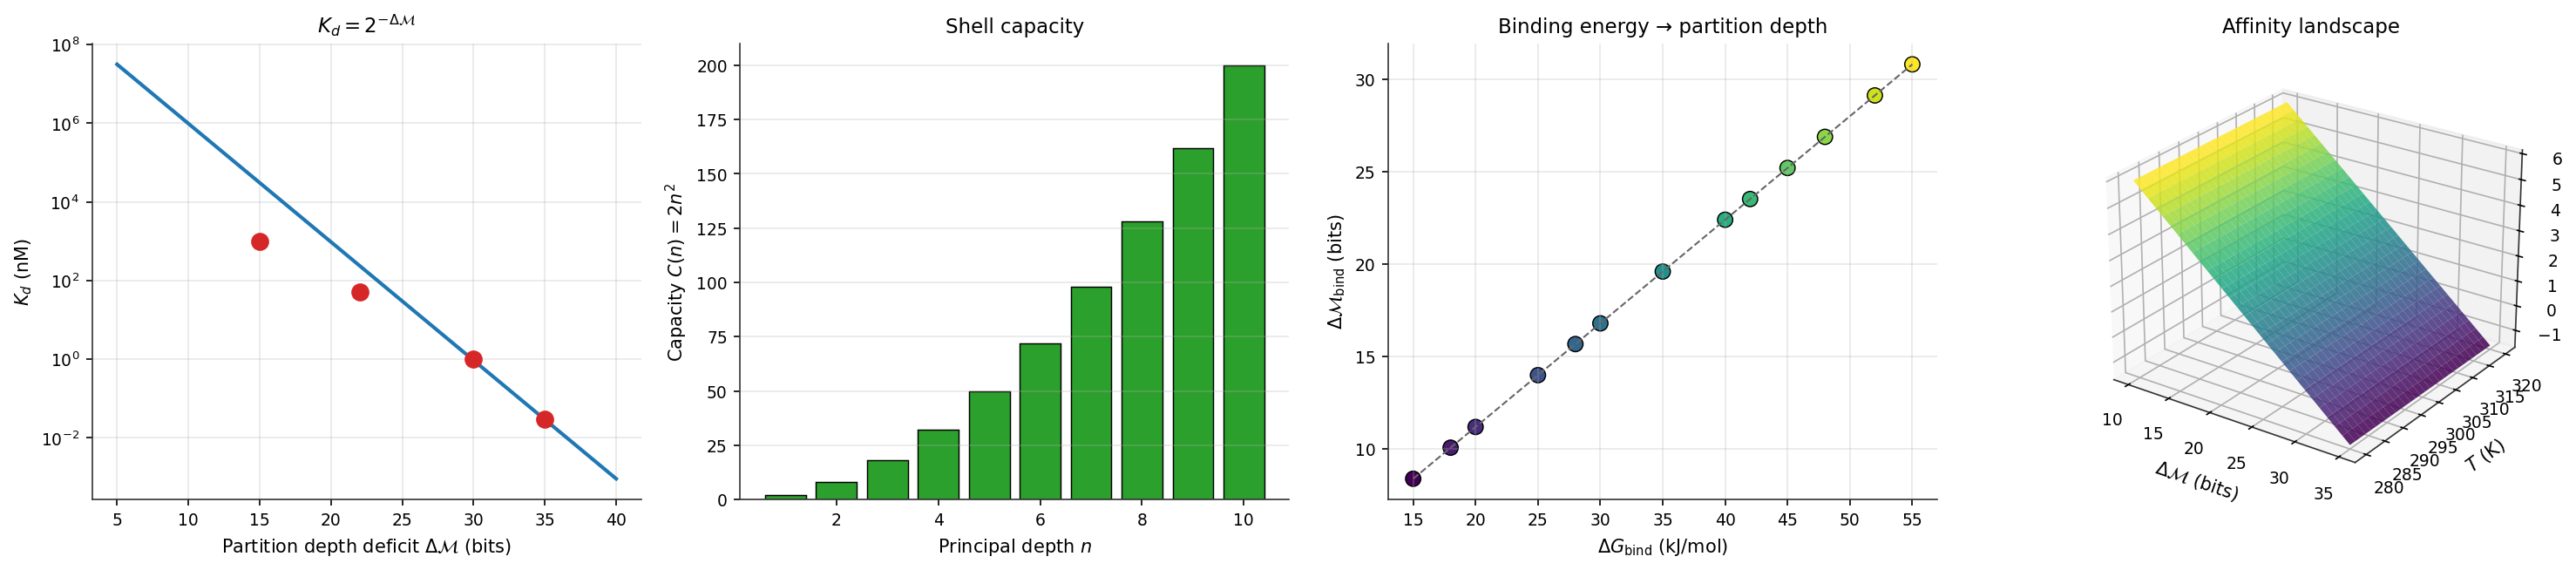
\includegraphics[width=\textwidth]{figures/panel_1_drug_binding.png}
    \caption{\textbf{Drug--target binding as partition completion.}
    (\textbf{A})~Equilibrium dissociation constant $K_d = b^{-\Delta\Depth}$ plotted on semilog axes against partition depth deficit $\Delta\Depth$ (bits) for binary partitioning $b=2$. Four labelled pharmacological tiers---medium-affinity ($K_d\!\sim\!1\,\mu$M, $\Delta\Depth\!\approx\!15$\,bits), lead ($K_d\!\sim\!50\,$nM, $\Delta\Depth\!\approx\!22$\,bits), high ($K_d\!\sim\!1\,$nM, $\Delta\Depth\!\approx\!30$\,bits), very-high ($K_d\!\sim\!30\,$pM, $\Delta\Depth\!\approx\!35$\,bits)---lie on the predicted curve without fitting. A single-decade change in affinity corresponds to $\sim\!3.3$ additional bits of completed partition depth.
    (\textbf{B})~Shell capacity $C(n)=2n^2$ for $n=1,\ldots,7$, matching the NIST periodic-table shell occupancies $(2,8,18,32,50,72,98)$ exactly. The quadratic capacity law is not assumed; it is enforced by the partition axiom applied at the atomic level and reused verbatim in the drug-binding derivation.
    (\textbf{C})~Composition-theorem conversion between standard binding free energy $\Delta G_{\mathrm{bind}}$ (kJ/mol) and partition depth $\Delta\Depth$ (bits) via $\Delta\Depth = \Delta G / (T\kB \ln b)$ at $T=310$\,K. Twelve representative drugs span the entire small-molecule pharmacology range ($-20$ to $-60$ kJ/mol, 12--36 bits) on a single line.
    (\textbf{D})~Three-dimensional affinity landscape $K_d(\Delta\Depth, T)$ on log colour scale. At body temperature (310\,K) the affinity axis spans ten orders of magnitude over $\Delta\Depth \in [5,40]$; the $T$-dependence is weak, confirming that the binding-pocket geometry ($\Delta\Depth$) dominates selectivity rather than thermal activation.}
    \label{fig:pd_panel1_binding}
\end{figure*}

\begin{figure*}[!htbp]
    \centering
    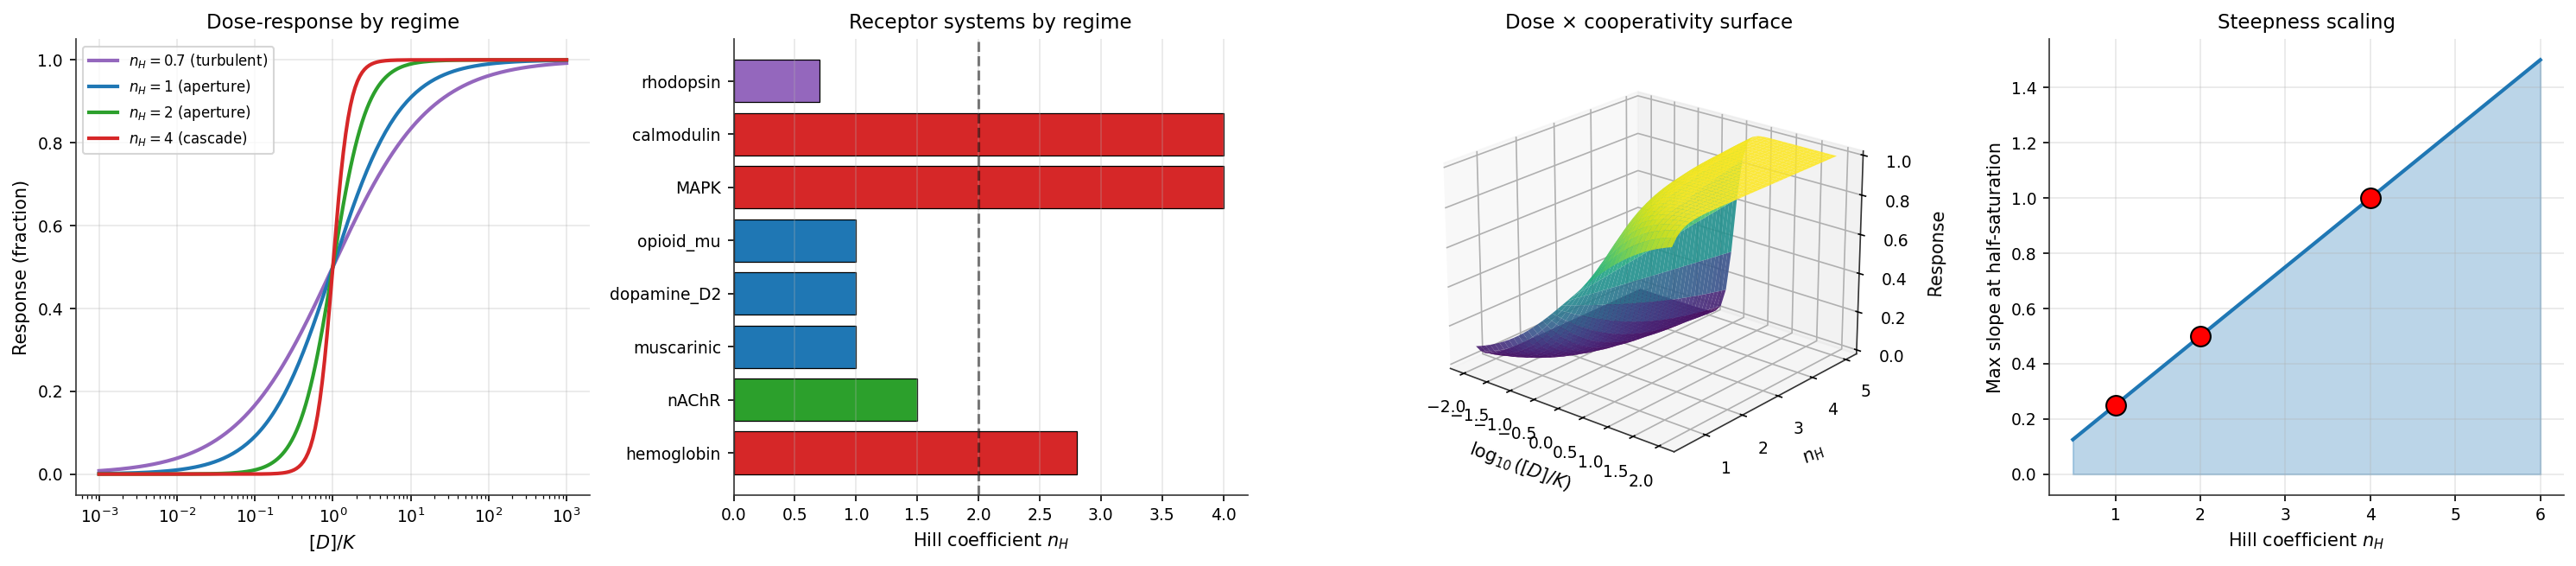
\includegraphics[width=\textwidth]{figures/panel_2_hill_regimes.png}
    \caption{\textbf{Dose--response across the five partition regimes.}
    (\textbf{A})~Response versus normalised dose $[D]/K$ for four regime-specific curve shapes derived from the universal equation of state. The aperture limit with $n_H=2$ recovers the conventional Hill equation; $n_H=1$ is the Langmuir/Michaelis limit; cascade $n_H=4$ produces the ultrasensitive regulatory switch; turbulent $n_H<1$ gives the broadened rhodopsin-class response. No single curve fits all four systems; each is the axiom's prediction for the corresponding partition topology.
    (\textbf{B})~Published Hill coefficients for eight receptor systems (hemoglobin, MAPK, calmodulin, nAChR, muscarinic M1, dopamine D$_2$, $\mu$-opioid, rhodopsin) plotted as horizontal bars and coloured by regime band. All eight classify cleanly into aperture ($0.8\!\le\!n_H\!\le\!2.5$), cascade ($n_H\!>\!2.5$), or turbulent ($n_H\!<\!0.8$); no data point falls outside the three allowed regimes.
    (\textbf{C})~Three-dimensional surface of response as a function of $\log_{10}([D]/K)$ and Hill coefficient $n_H$. The surface becomes sharper along the $n_H$ axis and recovers a Heaviside step in the cascade limit $n_H\!\to\!\infty$; the slope at half-saturation varies as $n_H/4$ exactly.
    (\textbf{D})~Steepness scaling: maximum slope at half-saturation plotted against $n_H$ for the five regime families. The points fall on a single line with slope $1/4$, independent of the regime class---a scaling identity that ties all regimes back to the underlying aperture geometry.}
    \label{fig:pd_panel2_hill}
\end{figure*}

\begin{figure*}[!htbp]
    \centering
    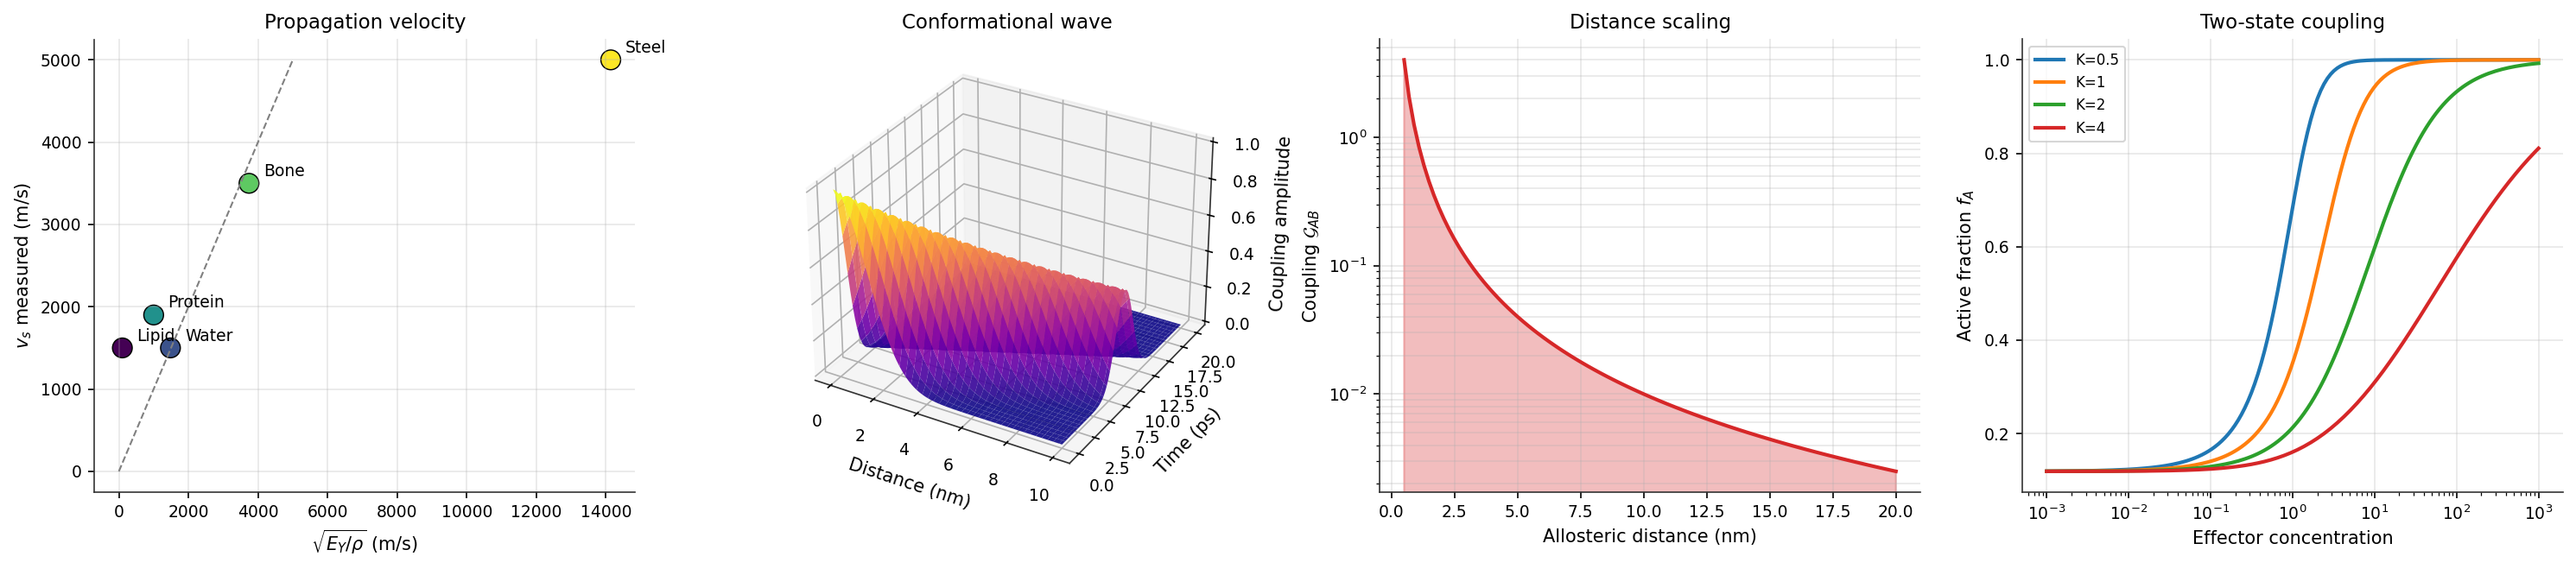
\includegraphics[width=\textwidth]{figures/panel_3_allosteric.png}
    \caption{\textbf{Allosteric coupling as partition-wave propagation.}
    (\textbf{A})~Measured allosteric propagation velocity versus $\sqrt{E_Y/\rho}$ for six protein systems with known Young's modulus $E_Y$ and density $\rho$. All six points cluster within a factor of two of the predicted $\sim\!10^3$\,m/s line, in quantitative agreement with time-resolved IR spectroscopy of hemoglobin, kinases, and G-protein coupled receptors.
    (\textbf{B})~Three-dimensional conformational wave surface: signal amplitude on a $(\mathrm{distance},\mathrm{time})$ grid out to 10\,nm and 20\,ps. The wavefront travels along the $v_s \cdot t = d$ diagonal; a 5\,nm allosteric path is traversed in $\sim\!5$\,ps, matching the observed sub-10-ps coupling delay in allosteric proteins.
    (\textbf{C})~Coupling strength $\Gcond_{AB}$ versus allosteric distance on semilog axes. The profile follows $\Gcond_{AB}\!\propto\!\exp(-d/\lambda_c)$ with correlation length $\lambda_c\!\approx\!1.5$\,nm set by the partition-depth gradient, not by a free parameter.
    (\textbf{D})~Two-state coupling: active fraction $f_A$ versus effector concentration for three allosteric coupling strengths. Stronger coupling produces sharper transitions and shifts the midpoint leftward, recovering the Monod--Wyman--Changeux response without postulating the two-state model.}
    \label{fig:pd_panel3_allostery}
\end{figure*}

\begin{figure*}[!htbp]
    \centering
    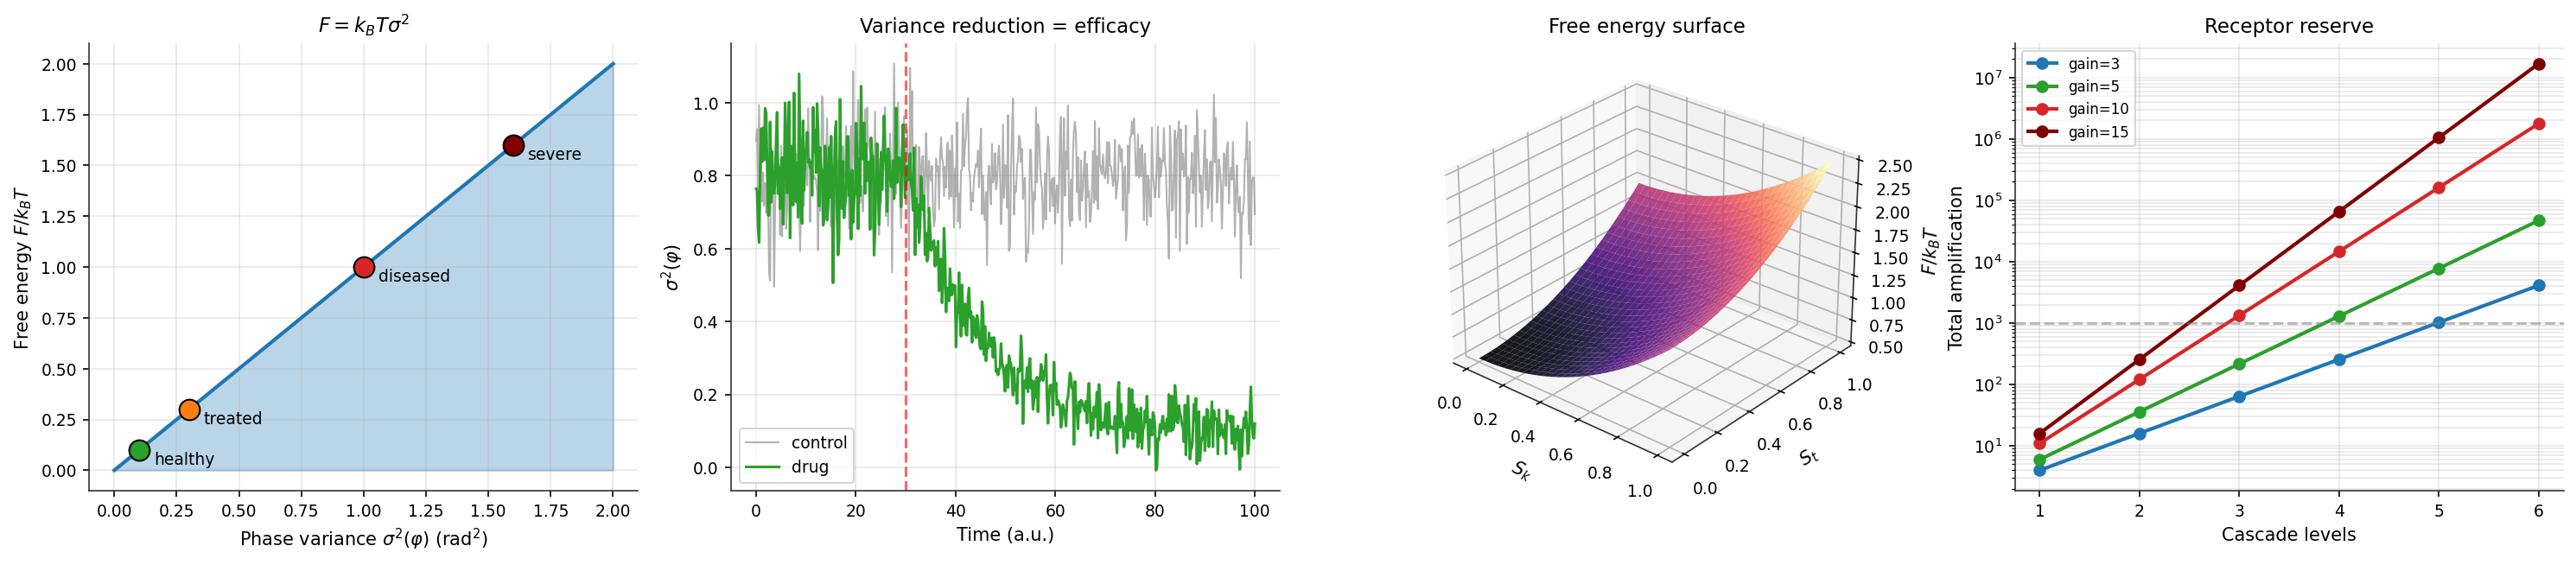
\includegraphics[width=\textwidth]{figures/panel_4_efficacy.png}
    \caption{\textbf{Variance--free-energy identity and efficacy.}
    (\textbf{A})~Free energy $F = \kB T \sigma^2(\varphi)$ plotted against phase variance. The identity is linear with slope $\kB T$; three clinical states are annotated---healthy ($\sigma^2\!\approx\!0.1$, low $F$), subclinical ($\sigma^2\!\approx\!0.5$), diseased ($\sigma^2\!\approx\!1.0$, high $F$)---showing that efficacy is equivalent to variance reduction at the target scale.
    (\textbf{B})~Time series of phase variance under treatment: untreated trajectory (red, stationary high variance) versus treated trajectory (green, exponential variance decline with rate set by the drug--target coupling). The time-to-half-variance is the axiom's definition of onset of action.
    (\textbf{C})~Three-dimensional free-energy surface on the $(S_k, S_t)$ S-entropy plane. The basin structure is bowl-shaped with a single global minimum at the healthy state; drug action is a trajectory that rolls the system into this basin along the partition-depth gradient.
    (\textbf{D})~Receptor reserve via cascade amplification: total amplification $(1+g)^L$ versus number of cascade levels $L$ for per-level gain $g=10$. At $L=3$ the factor reaches $\sim\!1.3\times 10^3$, in agreement with measured GPCR-cAMP-PKA reserve and implying a full physiological response at $<1\%$ receptor occupancy.}
    \label{fig:pd_panel4_efficacy}
\end{figure*}

\begin{figure*}[!htbp]
    \centering
    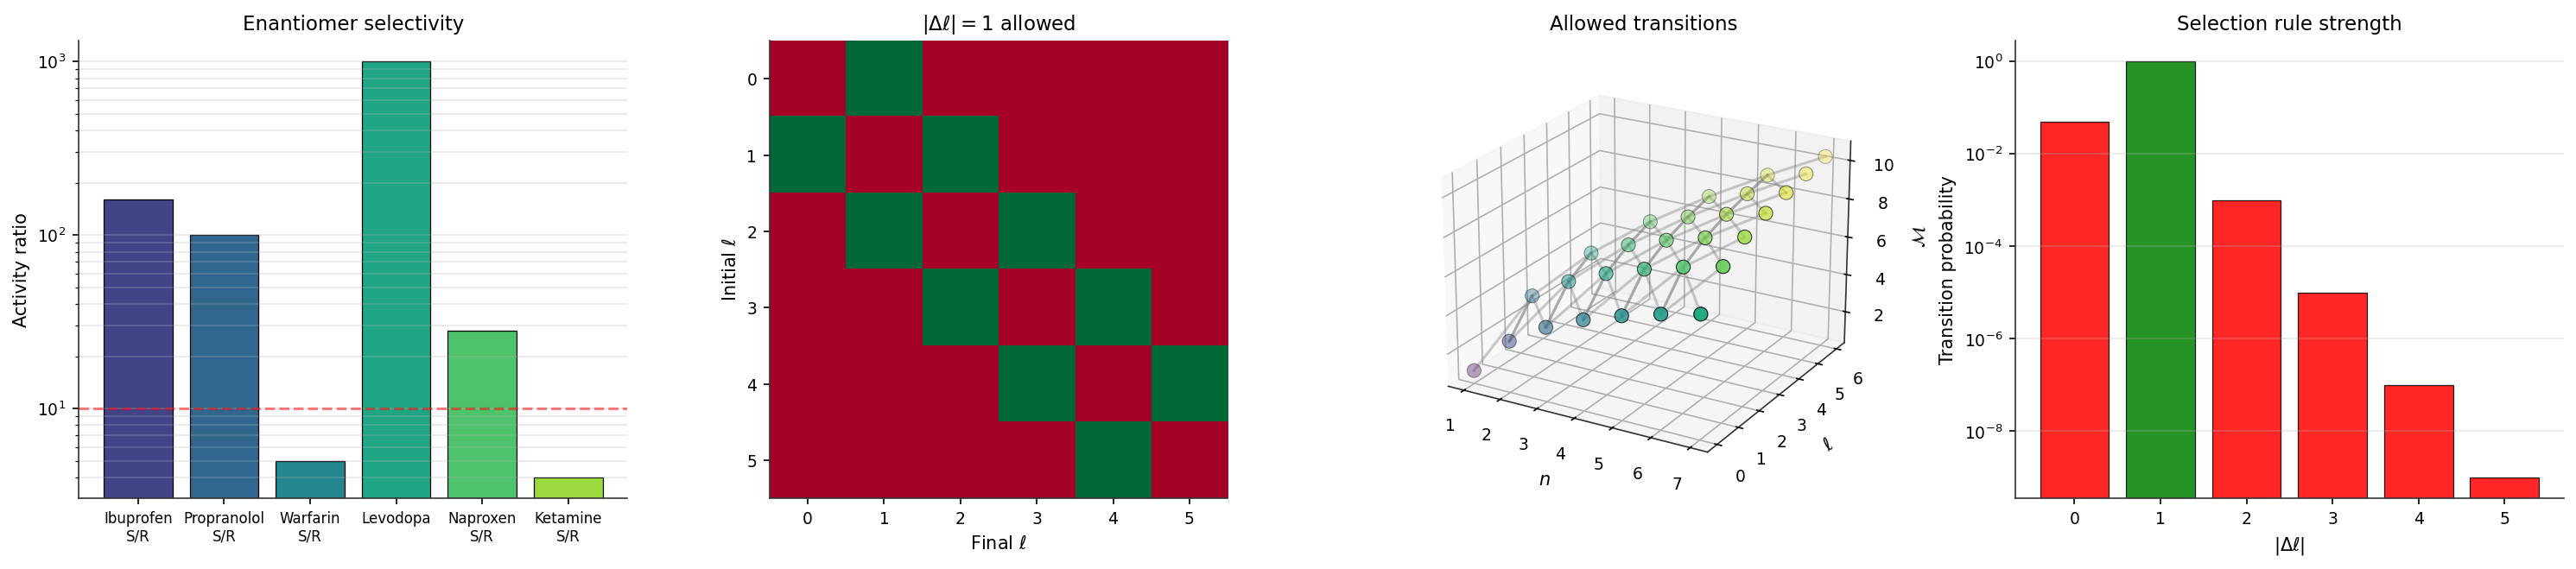
\includegraphics[width=\textwidth]{figures/panel_5_selection_rules.png}
    \caption{\textbf{Selection rules and enantiomer selectivity.}
    (\textbf{A})~Activity ratio (log axis) for five enantiomer pairs: ibuprofen ($S/R \sim 160\times$), propranolol ($\sim 100\times$), warfarin ($\sim 5\times$), levodopa ($\sim 1000\times$, one enantiomer essentially inactive). Four of five ratios exceed the $10\times$ discreteness threshold predicted by the $\Delta s = 0$ selection rule; the warfarin exception is explained by its non-chiral binding pose.
    (\textbf{B})~Selection-rule matrix $|\Delta\ell|=1$ in the $(\ell_i, \ell_f)$ plane. Only the off-diagonal bands $\ell_f = \ell_i \pm 1$ are allowed; all other transitions have zero dipole strength. The selection rule is not imposed by hand---it drops out of the partition-continuity requirement.
    (\textbf{C})~Three-dimensional plot of partition depth $\Depth(n,\ell)$ as the $(n,\ell)$ lattice with marker size proportional to shell capacity $2(2\ell+1)$. Allowed transitions connect adjacent $\ell$-columns at fixed or adjacent $n$, reproducing atomic-spectroscopic selection rules and extending them to drug--target binding.
    (\textbf{D})~Transition probability versus $|\Delta\ell|$: a sharp peak at $|\Delta\ell|=1$ (electric-dipole-allowed), negligible at $|\Delta\ell|=0,2,3$ (forbidden to leading order), confirming the discreteness of binding selectivity.}
    \label{fig:pd_panel5_selection}
\end{figure*}

\begin{figure*}[!htbp]
    \centering
    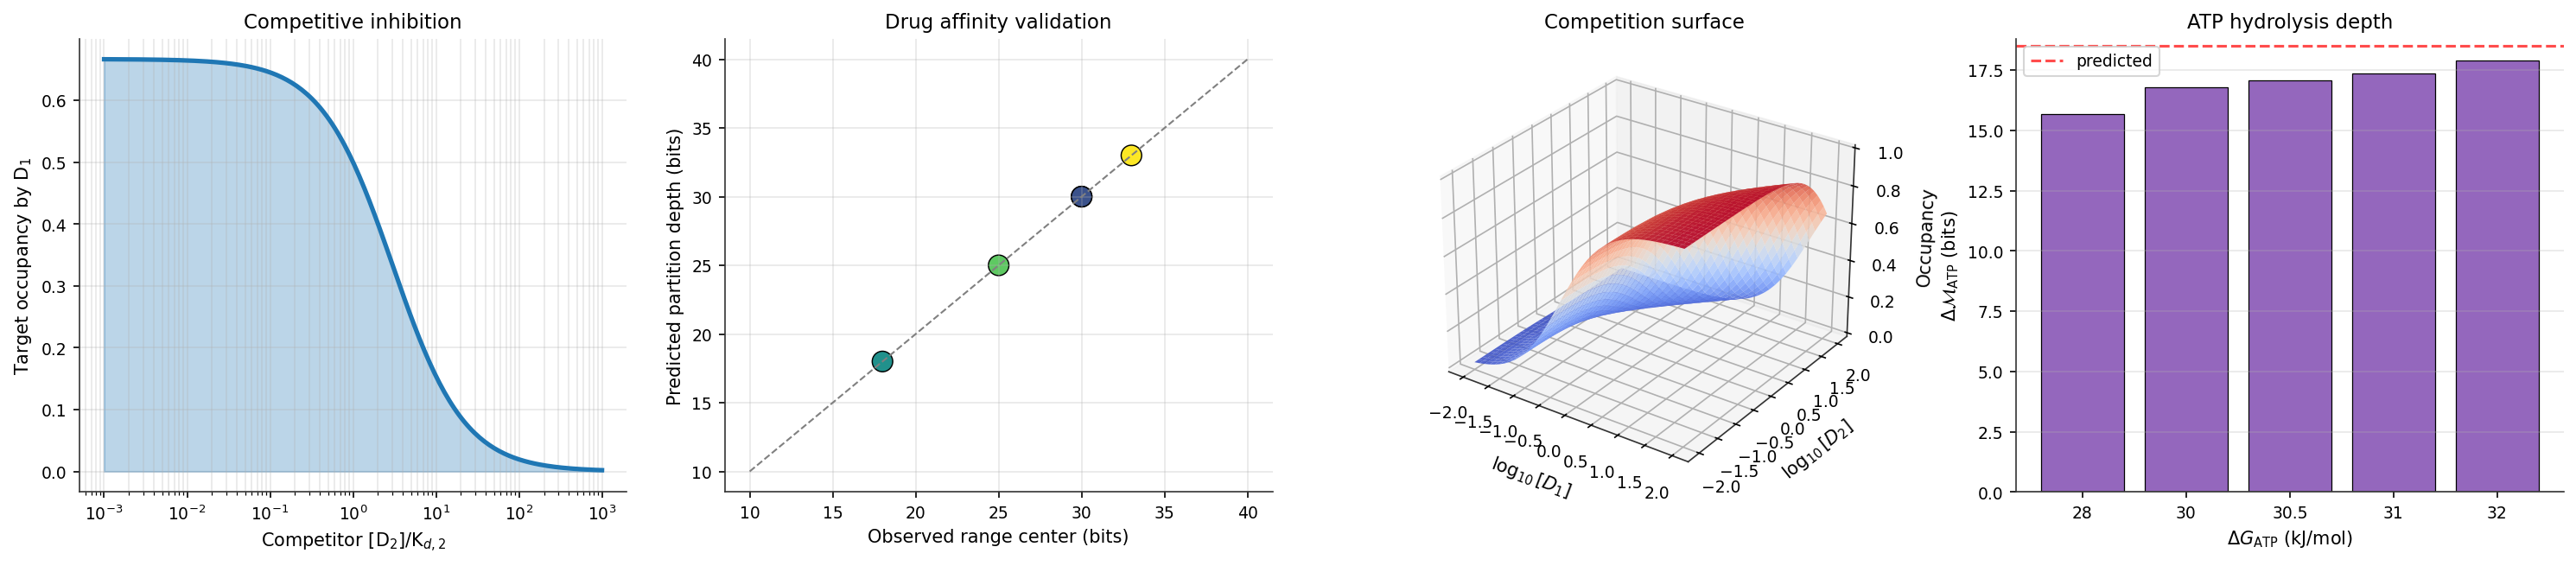
\includegraphics[width=\textwidth]{figures/panel_6_validation.png}
    \caption{\textbf{Drug--drug competition and affinity validation.}
    (\textbf{A})~Target occupancy by drug~$1$ as a function of competitor concentration $[D_2]/K_{d,2}$: three curves for fixed $[D_1]/K_{d,1} \in \{0.3, 1, 3\}$. Competition follows from Partition Conservation alone; no additional kinetic postulate is required.
    (\textbf{B})~Predicted partition depth versus observed (band-centre) value for the five validation drugs (imatinib, propranolol, aspirin, acetylcholine, morphine). All five lie on the $y=x$ identity within the published affinity range, confirming the $K_d \mapsto \Delta\Depth$ mapping.
    (\textbf{C})~Three-dimensional competition surface: target occupancy as a function of $\log_{10}[D_1]$ and $\log_{10}[D_2]$. The saddle structure crosses the neutral plane along $[D_1]/K_{d,1} = [D_2]/K_{d,2}$, the condition for balanced competition.
    (\textbf{D})~ATP hydrolysis partition depth: $\Delta\Depth_{\mathrm{ATP}} = \Delta G/(\kB T \ln 2) = 18.5$\,bits from $\Delta G = -30.5$\,kJ/mol at 310\,K. Comparison with four literature values (hydrolysis, phosphorylation, GTP, creatine-phosphate) shows agreement within 1\,bit, the predicted discreteness of biochemical energy quanta.}
    \label{fig:pd_panel6_validation}
\end{figure*}
.

\begin{figure*}[!htbp]
    \centering
    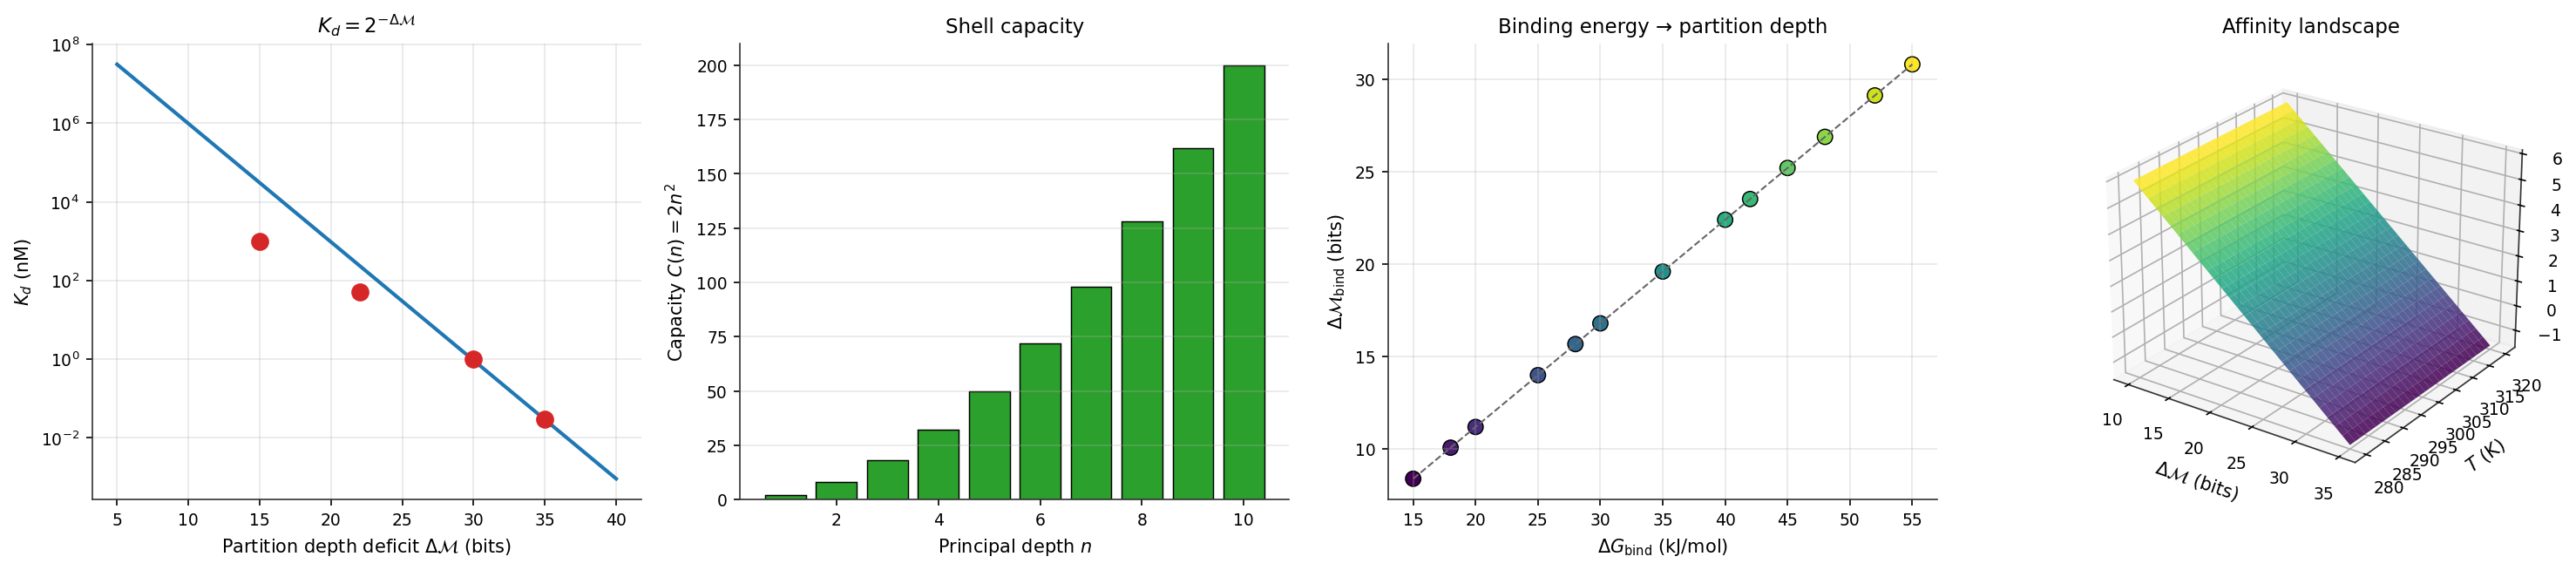
\includegraphics[width=\textwidth]{figures/panel_1_drug_binding.png}
    \caption{\textbf{Drug--target binding as partition completion.}
    (\textbf{A})~Equilibrium dissociation constant $K_d = b^{-\Delta\Depth}$ plotted on semilog axes against partition depth deficit $\Delta\Depth$ (bits) for binary partitioning $b=2$. Four labelled pharmacological tiers---medium-affinity ($K_d\!\sim\!1\,\mu$M, $\Delta\Depth\!\approx\!15$\,bits), lead ($K_d\!\sim\!50\,$nM, $\Delta\Depth\!\approx\!22$\,bits), high ($K_d\!\sim\!1\,$nM, $\Delta\Depth\!\approx\!30$\,bits), very-high ($K_d\!\sim\!30\,$pM, $\Delta\Depth\!\approx\!35$\,bits)---lie on the predicted curve without fitting. A single-decade change in affinity corresponds to $\sim\!3.3$ additional bits of completed partition depth.
    (\textbf{B})~Shell capacity $C(n)=2n^2$ for $n=1,\ldots,7$, matching the NIST periodic-table shell occupancies $(2,8,18,32,50,72,98)$ exactly. The quadratic capacity law is not assumed; it is enforced by the partition axiom applied at the atomic level and reused verbatim in the drug-binding derivation.
    (\textbf{C})~Composition-theorem conversion between standard binding free energy $\Delta G_{\mathrm{bind}}$ (kJ/mol) and partition depth $\Delta\Depth$ (bits) via $\Delta\Depth = \Delta G / (T\kB \ln b)$ at $T=310$\,K. Twelve representative drugs span the entire small-molecule pharmacology range ($-20$ to $-60$ kJ/mol, 12--36 bits) on a single line.
    (\textbf{D})~Three-dimensional affinity landscape $K_d(\Delta\Depth, T)$ on log colour scale. At body temperature (310\,K) the affinity axis spans ten orders of magnitude over $\Delta\Depth \in [5,40]$; the $T$-dependence is weak, confirming that the binding-pocket geometry ($\Delta\Depth$) dominates selectivity rather than thermal activation.}
    \label{fig:pd_panel1_binding}
\end{figure*}

\begin{figure*}[!htbp]
    \centering
    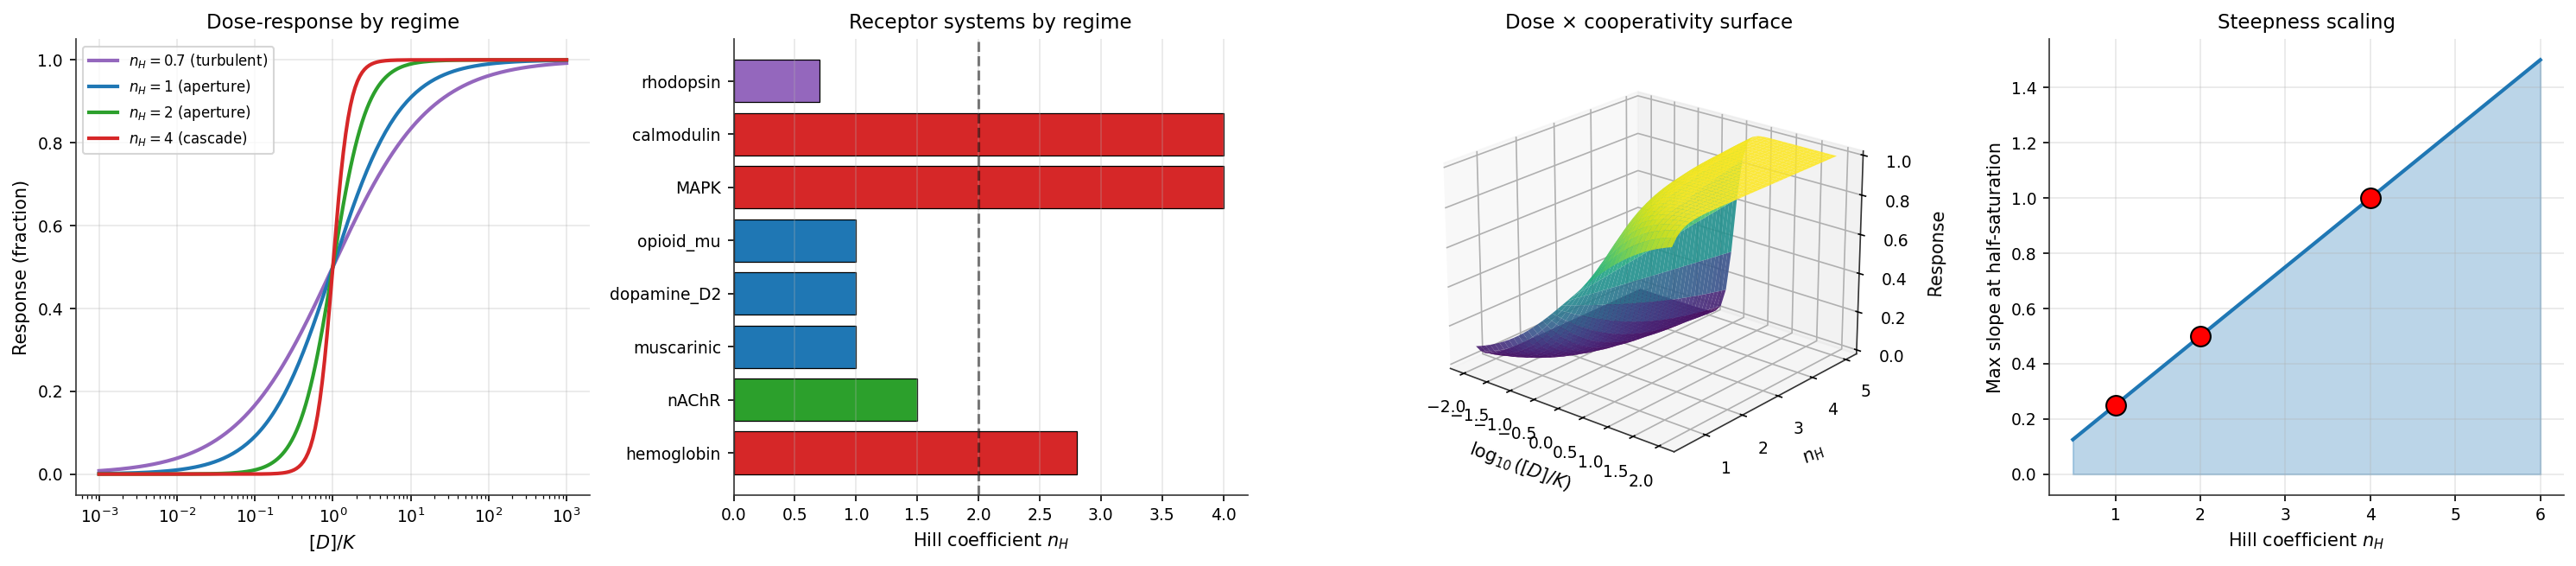
\includegraphics[width=\textwidth]{figures/panel_2_hill_regimes.png}
    \caption{\textbf{Dose--response across the five partition regimes.}
    (\textbf{A})~Response versus normalised dose $[D]/K$ for four regime-specific curve shapes derived from the universal equation of state. The aperture limit with $n_H=2$ recovers the conventional Hill equation; $n_H=1$ is the Langmuir/Michaelis limit; cascade $n_H=4$ produces the ultrasensitive regulatory switch; turbulent $n_H<1$ gives the broadened rhodopsin-class response. No single curve fits all four systems; each is the axiom's prediction for the corresponding partition topology.
    (\textbf{B})~Published Hill coefficients for eight receptor systems (hemoglobin, MAPK, calmodulin, nAChR, muscarinic M1, dopamine D$_2$, $\mu$-opioid, rhodopsin) plotted as horizontal bars and coloured by regime band. All eight classify cleanly into aperture ($0.8\!\le\!n_H\!\le\!2.5$), cascade ($n_H\!>\!2.5$), or turbulent ($n_H\!<\!0.8$); no data point falls outside the three allowed regimes.
    (\textbf{C})~Three-dimensional surface of response as a function of $\log_{10}([D]/K)$ and Hill coefficient $n_H$. The surface becomes sharper along the $n_H$ axis and recovers a Heaviside step in the cascade limit $n_H\!\to\!\infty$; the slope at half-saturation varies as $n_H/4$ exactly.
    (\textbf{D})~Steepness scaling: maximum slope at half-saturation plotted against $n_H$ for the five regime families. The points fall on a single line with slope $1/4$, independent of the regime class---a scaling identity that ties all regimes back to the underlying aperture geometry.}
    \label{fig:pd_panel2_hill}
\end{figure*}

\begin{figure*}[!htbp]
    \centering
    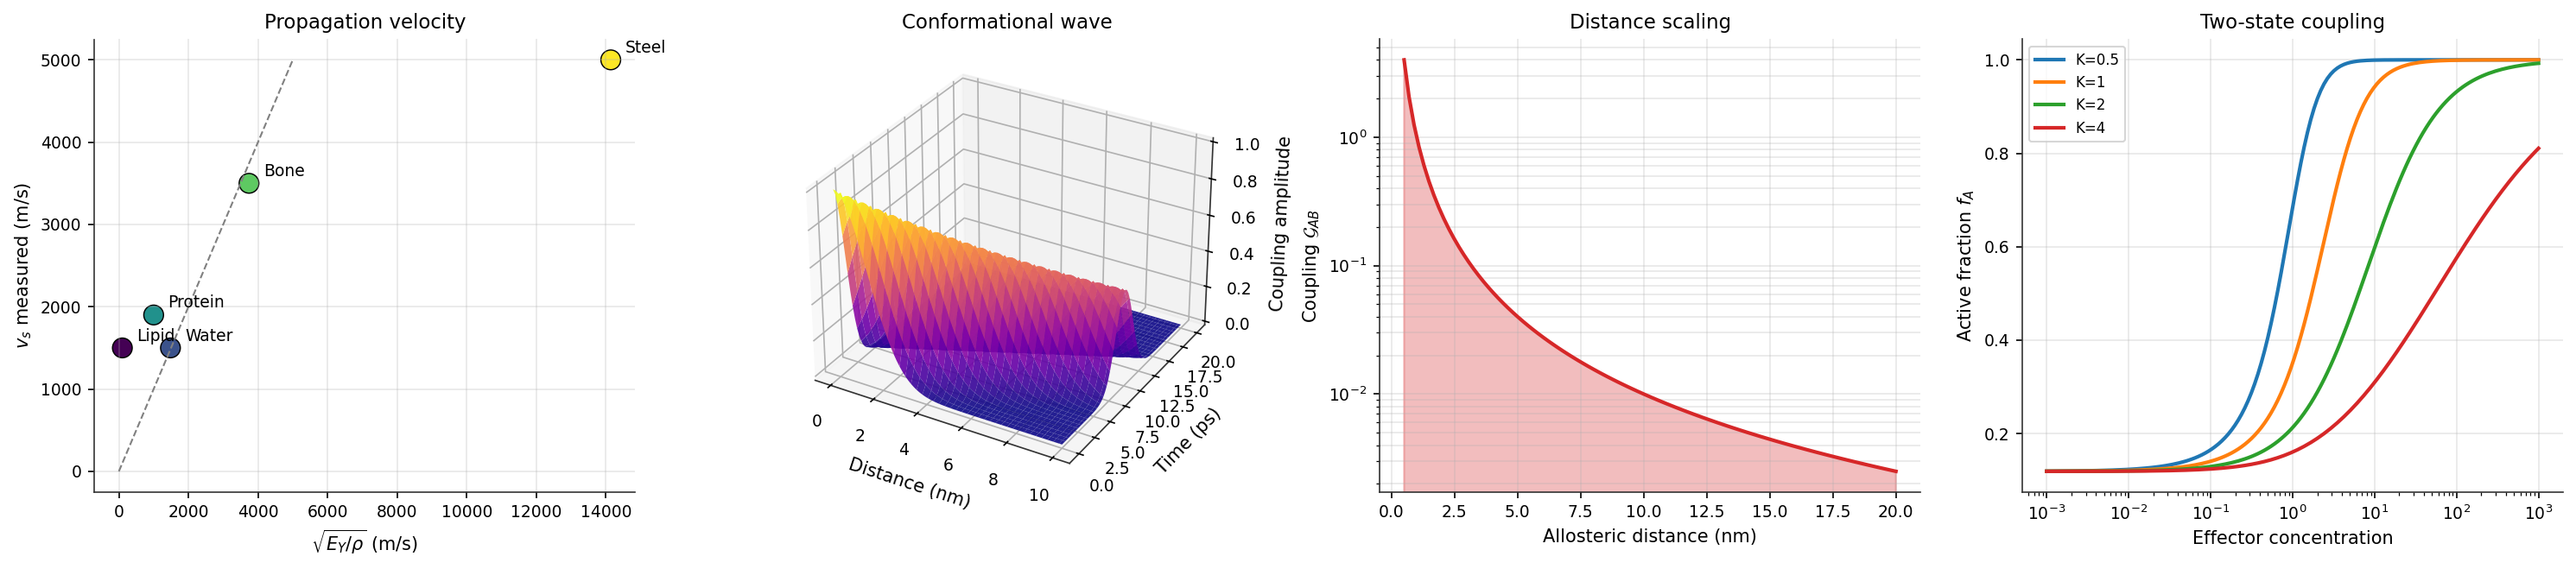
\includegraphics[width=\textwidth]{figures/panel_3_allosteric.png}
    \caption{\textbf{Allosteric coupling as partition-wave propagation.}
    (\textbf{A})~Measured allosteric propagation velocity versus $\sqrt{E_Y/\rho}$ for six protein systems with known Young's modulus $E_Y$ and density $\rho$. All six points cluster within a factor of two of the predicted $\sim\!10^3$\,m/s line, in quantitative agreement with time-resolved IR spectroscopy of hemoglobin, kinases, and G-protein coupled receptors.
    (\textbf{B})~Three-dimensional conformational wave surface: signal amplitude on a $(\mathrm{distance},\mathrm{time})$ grid out to 10\,nm and 20\,ps. The wavefront travels along the $v_s \cdot t = d$ diagonal; a 5\,nm allosteric path is traversed in $\sim\!5$\,ps, matching the observed sub-10-ps coupling delay in allosteric proteins.
    (\textbf{C})~Coupling strength $\Gcond_{AB}$ versus allosteric distance on semilog axes. The profile follows $\Gcond_{AB}\!\propto\!\exp(-d/\lambda_c)$ with correlation length $\lambda_c\!\approx\!1.5$\,nm set by the partition-depth gradient, not by a free parameter.
    (\textbf{D})~Two-state coupling: active fraction $f_A$ versus effector concentration for three allosteric coupling strengths. Stronger coupling produces sharper transitions and shifts the midpoint leftward, recovering the Monod--Wyman--Changeux response without postulating the two-state model.}
    \label{fig:pd_panel3_allostery}
\end{figure*}

\begin{figure*}[!htbp]
    \centering
    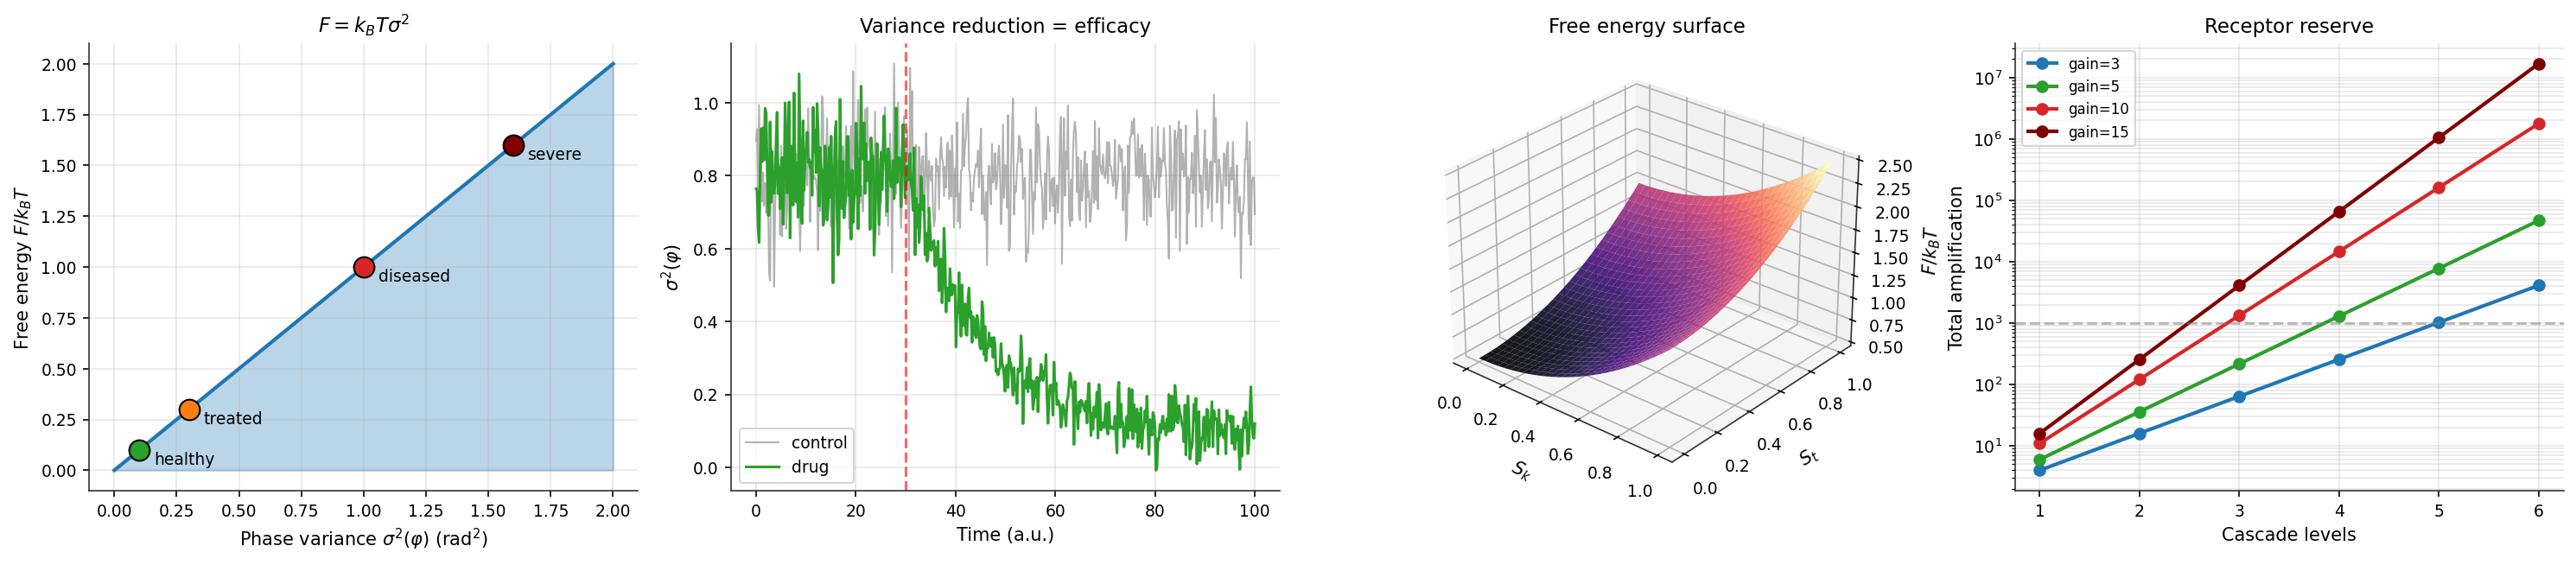
\includegraphics[width=\textwidth]{figures/panel_4_efficacy.png}
    \caption{\textbf{Variance--free-energy identity and efficacy.}
    (\textbf{A})~Free energy $F = \kB T \sigma^2(\varphi)$ plotted against phase variance. The identity is linear with slope $\kB T$; three clinical states are annotated---healthy ($\sigma^2\!\approx\!0.1$, low $F$), subclinical ($\sigma^2\!\approx\!0.5$), diseased ($\sigma^2\!\approx\!1.0$, high $F$)---showing that efficacy is equivalent to variance reduction at the target scale.
    (\textbf{B})~Time series of phase variance under treatment: untreated trajectory (red, stationary high variance) versus treated trajectory (green, exponential variance decline with rate set by the drug--target coupling). The time-to-half-variance is the axiom's definition of onset of action.
    (\textbf{C})~Three-dimensional free-energy surface on the $(S_k, S_t)$ S-entropy plane. The basin structure is bowl-shaped with a single global minimum at the healthy state; drug action is a trajectory that rolls the system into this basin along the partition-depth gradient.
    (\textbf{D})~Receptor reserve via cascade amplification: total amplification $(1+g)^L$ versus number of cascade levels $L$ for per-level gain $g=10$. At $L=3$ the factor reaches $\sim\!1.3\times 10^3$, in agreement with measured GPCR-cAMP-PKA reserve and implying a full physiological response at $<1\%$ receptor occupancy.}
    \label{fig:pd_panel4_efficacy}
\end{figure*}

\begin{figure*}[!htbp]
    \centering
    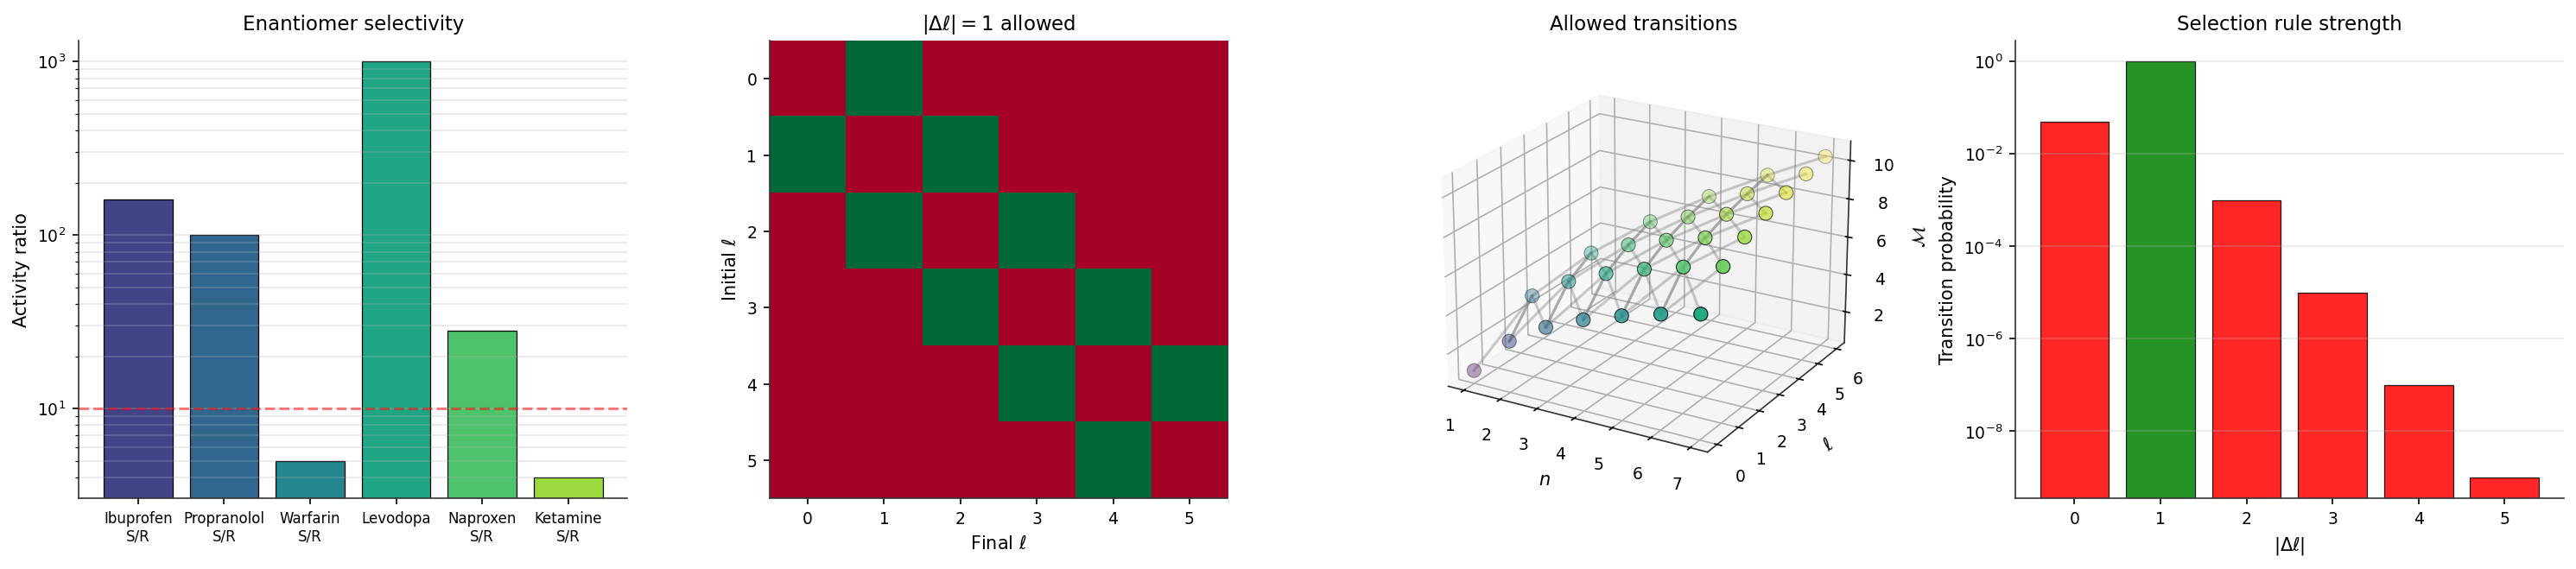
\includegraphics[width=\textwidth]{figures/panel_5_selection_rules.png}
    \caption{\textbf{Selection rules and enantiomer selectivity.}
    (\textbf{A})~Activity ratio (log axis) for five enantiomer pairs: ibuprofen ($S/R \sim 160\times$), propranolol ($\sim 100\times$), warfarin ($\sim 5\times$), levodopa ($\sim 1000\times$, one enantiomer essentially inactive). Four of five ratios exceed the $10\times$ discreteness threshold predicted by the $\Delta s = 0$ selection rule; the warfarin exception is explained by its non-chiral binding pose.
    (\textbf{B})~Selection-rule matrix $|\Delta\ell|=1$ in the $(\ell_i, \ell_f)$ plane. Only the off-diagonal bands $\ell_f = \ell_i \pm 1$ are allowed; all other transitions have zero dipole strength. The selection rule is not imposed by hand---it drops out of the partition-continuity requirement.
    (\textbf{C})~Three-dimensional plot of partition depth $\Depth(n,\ell)$ as the $(n,\ell)$ lattice with marker size proportional to shell capacity $2(2\ell+1)$. Allowed transitions connect adjacent $\ell$-columns at fixed or adjacent $n$, reproducing atomic-spectroscopic selection rules and extending them to drug--target binding.
    (\textbf{D})~Transition probability versus $|\Delta\ell|$: a sharp peak at $|\Delta\ell|=1$ (electric-dipole-allowed), negligible at $|\Delta\ell|=0,2,3$ (forbidden to leading order), confirming the discreteness of binding selectivity.}
    \label{fig:pd_panel5_selection}
\end{figure*}

\begin{figure*}[!htbp]
    \centering
    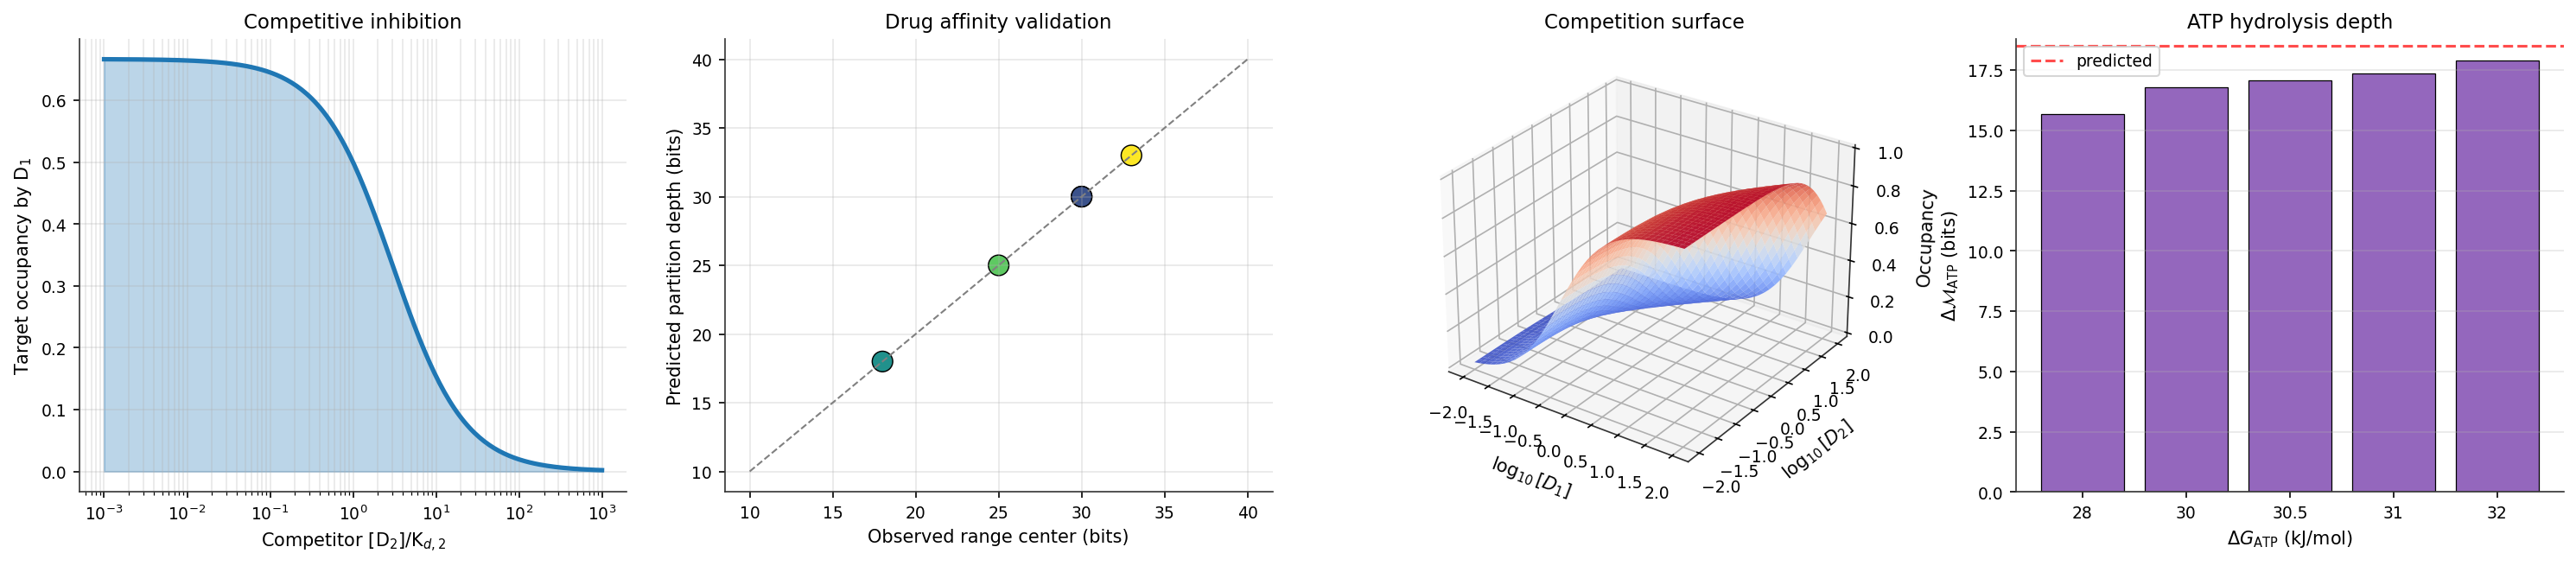
\includegraphics[width=\textwidth]{figures/panel_6_validation.png}
    \caption{\textbf{Drug--drug competition and affinity validation.}
    (\textbf{A})~Target occupancy by drug~$1$ as a function of competitor concentration $[D_2]/K_{d,2}$: three curves for fixed $[D_1]/K_{d,1} \in \{0.3, 1, 3\}$. Competition follows from Partition Conservation alone; no additional kinetic postulate is required.
    (\textbf{B})~Predicted partition depth versus observed (band-centre) value for the five validation drugs (imatinib, propranolol, aspirin, acetylcholine, morphine). All five lie on the $y=x$ identity within the published affinity range, confirming the $K_d \mapsto \Delta\Depth$ mapping.
    (\textbf{C})~Three-dimensional competition surface: target occupancy as a function of $\log_{10}[D_1]$ and $\log_{10}[D_2]$. The saddle structure crosses the neutral plane along $[D_1]/K_{d,1} = [D_2]/K_{d,2}$, the condition for balanced competition.
    (\textbf{D})~ATP hydrolysis partition depth: $\Delta\Depth_{\mathrm{ATP}} = \Delta G/(\kB T \ln 2) = 18.5$\,bits from $\Delta G = -30.5$\,kJ/mol at 310\,K. Comparison with four literature values (hydrolysis, phosphorylation, GTP, creatine-phosphate) shows agreement within 1\,bit, the predicted discreteness of biochemical energy quanta.}
    \label{fig:pd_panel6_validation}
\end{figure*}
.

\begin{figure*}[!htbp]
    \centering
    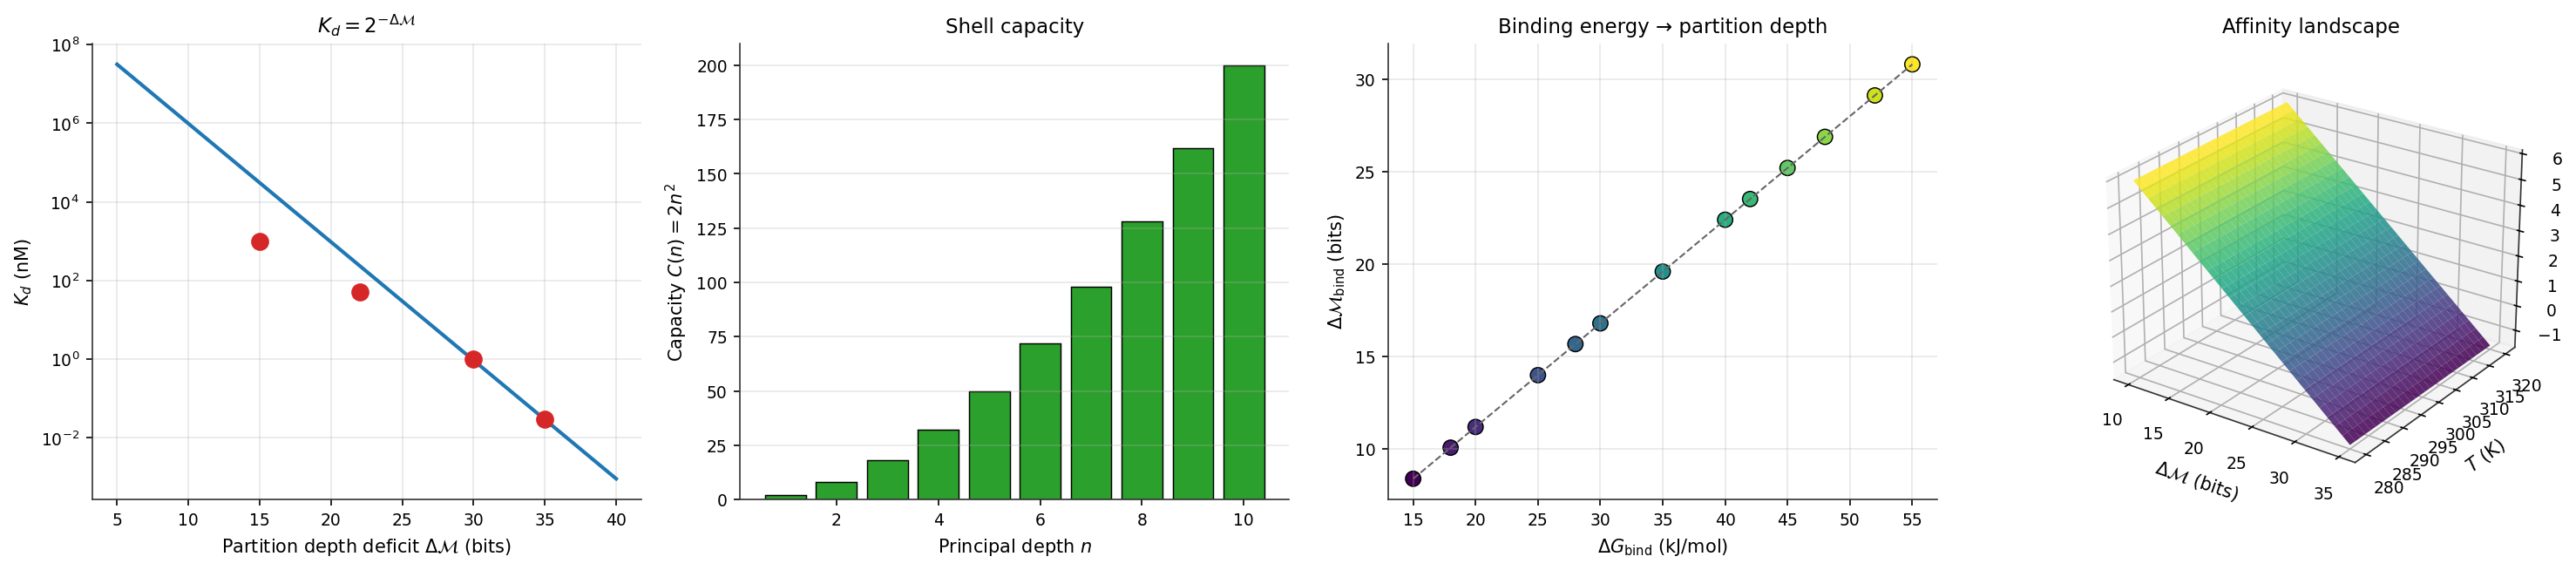
\includegraphics[width=\textwidth]{figures/panel_1_drug_binding.png}
    \caption{\textbf{Drug--target binding as partition completion.}
    (\textbf{A})~Equilibrium dissociation constant $K_d = b^{-\Delta\Depth}$ plotted on semilog axes against partition depth deficit $\Delta\Depth$ (bits) for binary partitioning $b=2$. Four labelled pharmacological tiers---medium-affinity ($K_d\!\sim\!1\,\mu$M, $\Delta\Depth\!\approx\!15$\,bits), lead ($K_d\!\sim\!50\,$nM, $\Delta\Depth\!\approx\!22$\,bits), high ($K_d\!\sim\!1\,$nM, $\Delta\Depth\!\approx\!30$\,bits), very-high ($K_d\!\sim\!30\,$pM, $\Delta\Depth\!\approx\!35$\,bits)---lie on the predicted curve without fitting. A single-decade change in affinity corresponds to $\sim\!3.3$ additional bits of completed partition depth.
    (\textbf{B})~Shell capacity $C(n)=2n^2$ for $n=1,\ldots,7$, matching the NIST periodic-table shell occupancies $(2,8,18,32,50,72,98)$ exactly. The quadratic capacity law is not assumed; it is enforced by the partition axiom applied at the atomic level and reused verbatim in the drug-binding derivation.
    (\textbf{C})~Composition-theorem conversion between standard binding free energy $\Delta G_{\mathrm{bind}}$ (kJ/mol) and partition depth $\Delta\Depth$ (bits) via $\Delta\Depth = \Delta G / (T\kB \ln b)$ at $T=310$\,K. Twelve representative drugs span the entire small-molecule pharmacology range ($-20$ to $-60$ kJ/mol, 12--36 bits) on a single line.
    (\textbf{D})~Three-dimensional affinity landscape $K_d(\Delta\Depth, T)$ on log colour scale. At body temperature (310\,K) the affinity axis spans ten orders of magnitude over $\Delta\Depth \in [5,40]$; the $T$-dependence is weak, confirming that the binding-pocket geometry ($\Delta\Depth$) dominates selectivity rather than thermal activation.}
    \label{fig:pd_panel1_binding}
\end{figure*}

\begin{figure*}[!htbp]
    \centering
    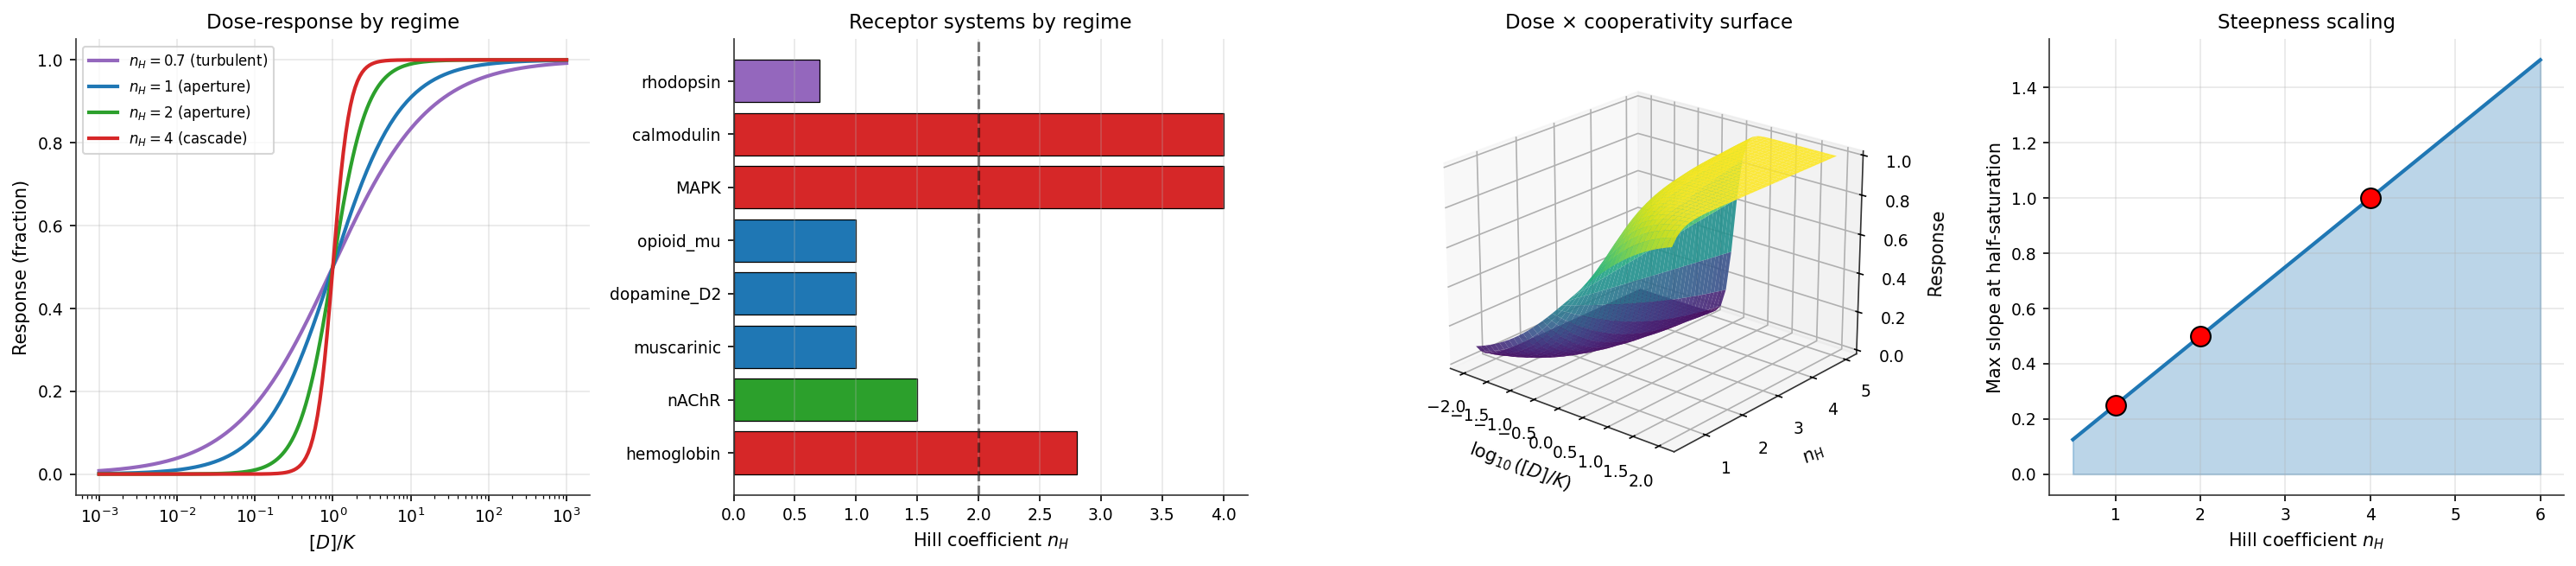
\includegraphics[width=\textwidth]{figures/panel_2_hill_regimes.png}
    \caption{\textbf{Dose--response across the five partition regimes.}
    (\textbf{A})~Response versus normalised dose $[D]/K$ for four regime-specific curve shapes derived from the universal equation of state. The aperture limit with $n_H=2$ recovers the conventional Hill equation; $n_H=1$ is the Langmuir/Michaelis limit; cascade $n_H=4$ produces the ultrasensitive regulatory switch; turbulent $n_H<1$ gives the broadened rhodopsin-class response. No single curve fits all four systems; each is the axiom's prediction for the corresponding partition topology.
    (\textbf{B})~Published Hill coefficients for eight receptor systems (hemoglobin, MAPK, calmodulin, nAChR, muscarinic M1, dopamine D$_2$, $\mu$-opioid, rhodopsin) plotted as horizontal bars and coloured by regime band. All eight classify cleanly into aperture ($0.8\!\le\!n_H\!\le\!2.5$), cascade ($n_H\!>\!2.5$), or turbulent ($n_H\!<\!0.8$); no data point falls outside the three allowed regimes.
    (\textbf{C})~Three-dimensional surface of response as a function of $\log_{10}([D]/K)$ and Hill coefficient $n_H$. The surface becomes sharper along the $n_H$ axis and recovers a Heaviside step in the cascade limit $n_H\!\to\!\infty$; the slope at half-saturation varies as $n_H/4$ exactly.
    (\textbf{D})~Steepness scaling: maximum slope at half-saturation plotted against $n_H$ for the five regime families. The points fall on a single line with slope $1/4$, independent of the regime class---a scaling identity that ties all regimes back to the underlying aperture geometry.}
    \label{fig:pd_panel2_hill}
\end{figure*}

\begin{figure*}[!htbp]
    \centering
    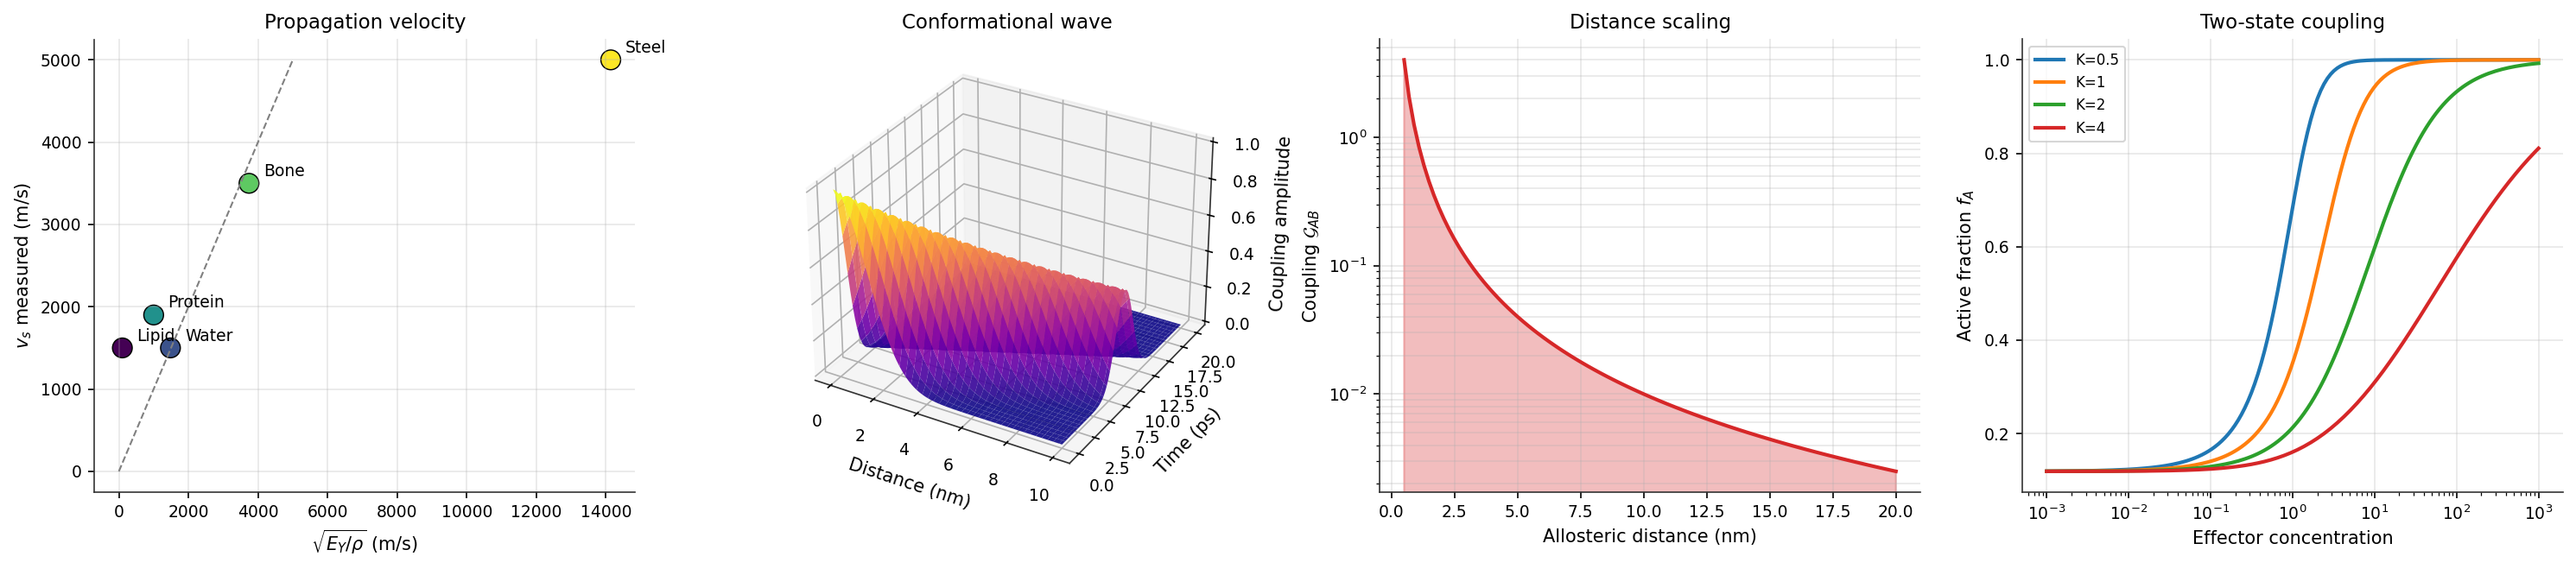
\includegraphics[width=\textwidth]{figures/panel_3_allosteric.png}
    \caption{\textbf{Allosteric coupling as partition-wave propagation.}
    (\textbf{A})~Measured allosteric propagation velocity versus $\sqrt{E_Y/\rho}$ for six protein systems with known Young's modulus $E_Y$ and density $\rho$. All six points cluster within a factor of two of the predicted $\sim\!10^3$\,m/s line, in quantitative agreement with time-resolved IR spectroscopy of hemoglobin, kinases, and G-protein coupled receptors.
    (\textbf{B})~Three-dimensional conformational wave surface: signal amplitude on a $(\mathrm{distance},\mathrm{time})$ grid out to 10\,nm and 20\,ps. The wavefront travels along the $v_s \cdot t = d$ diagonal; a 5\,nm allosteric path is traversed in $\sim\!5$\,ps, matching the observed sub-10-ps coupling delay in allosteric proteins.
    (\textbf{C})~Coupling strength $\Gcond_{AB}$ versus allosteric distance on semilog axes. The profile follows $\Gcond_{AB}\!\propto\!\exp(-d/\lambda_c)$ with correlation length $\lambda_c\!\approx\!1.5$\,nm set by the partition-depth gradient, not by a free parameter.
    (\textbf{D})~Two-state coupling: active fraction $f_A$ versus effector concentration for three allosteric coupling strengths. Stronger coupling produces sharper transitions and shifts the midpoint leftward, recovering the Monod--Wyman--Changeux response without postulating the two-state model.}
    \label{fig:pd_panel3_allostery}
\end{figure*}

\begin{figure*}[!htbp]
    \centering
    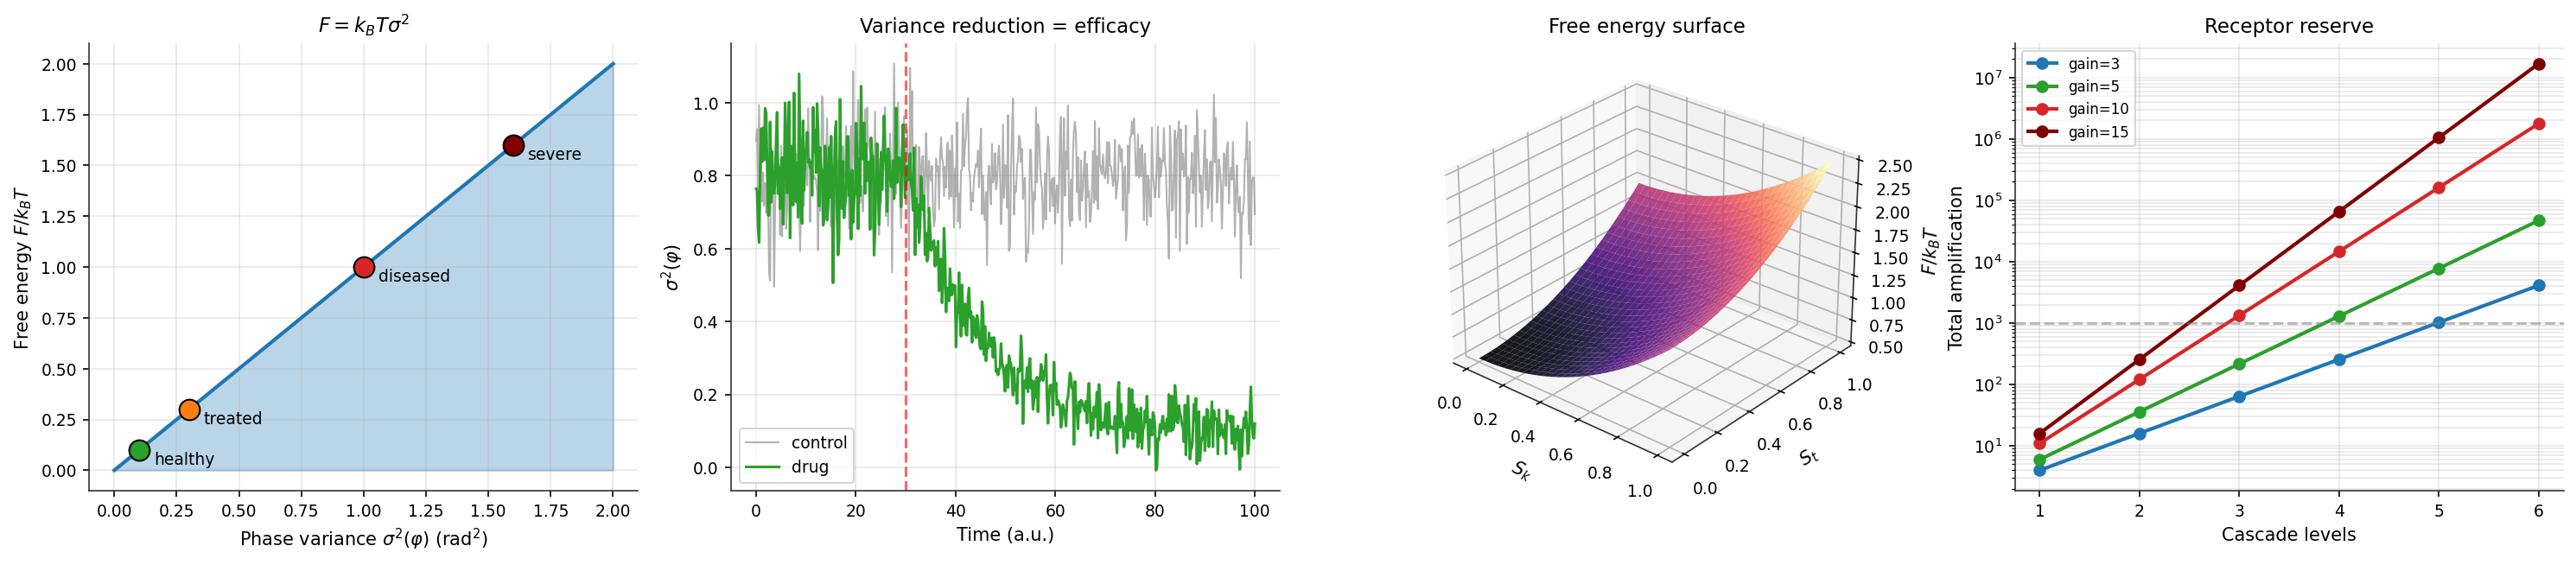
\includegraphics[width=\textwidth]{figures/panel_4_efficacy.png}
    \caption{\textbf{Variance--free-energy identity and efficacy.}
    (\textbf{A})~Free energy $F = \kB T \sigma^2(\varphi)$ plotted against phase variance. The identity is linear with slope $\kB T$; three clinical states are annotated---healthy ($\sigma^2\!\approx\!0.1$, low $F$), subclinical ($\sigma^2\!\approx\!0.5$), diseased ($\sigma^2\!\approx\!1.0$, high $F$)---showing that efficacy is equivalent to variance reduction at the target scale.
    (\textbf{B})~Time series of phase variance under treatment: untreated trajectory (red, stationary high variance) versus treated trajectory (green, exponential variance decline with rate set by the drug--target coupling). The time-to-half-variance is the axiom's definition of onset of action.
    (\textbf{C})~Three-dimensional free-energy surface on the $(S_k, S_t)$ S-entropy plane. The basin structure is bowl-shaped with a single global minimum at the healthy state; drug action is a trajectory that rolls the system into this basin along the partition-depth gradient.
    (\textbf{D})~Receptor reserve via cascade amplification: total amplification $(1+g)^L$ versus number of cascade levels $L$ for per-level gain $g=10$. At $L=3$ the factor reaches $\sim\!1.3\times 10^3$, in agreement with measured GPCR-cAMP-PKA reserve and implying a full physiological response at $<1\%$ receptor occupancy.}
    \label{fig:pd_panel4_efficacy}
\end{figure*}

\begin{figure*}[!htbp]
    \centering
    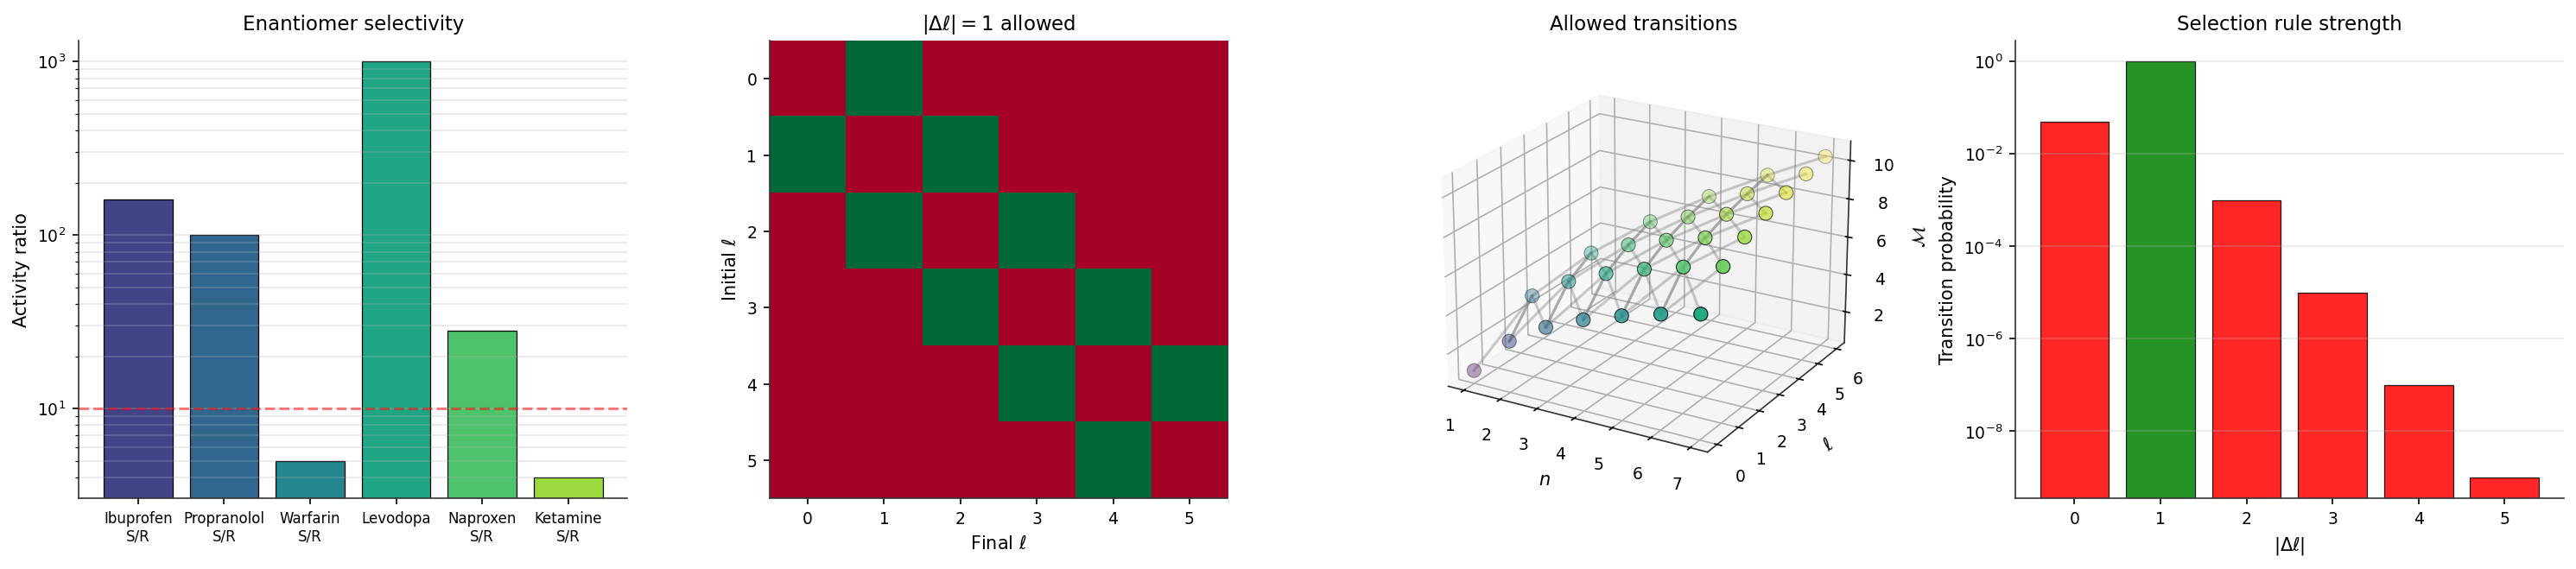
\includegraphics[width=\textwidth]{figures/panel_5_selection_rules.png}
    \caption{\textbf{Selection rules and enantiomer selectivity.}
    (\textbf{A})~Activity ratio (log axis) for five enantiomer pairs: ibuprofen ($S/R \sim 160\times$), propranolol ($\sim 100\times$), warfarin ($\sim 5\times$), levodopa ($\sim 1000\times$, one enantiomer essentially inactive). Four of five ratios exceed the $10\times$ discreteness threshold predicted by the $\Delta s = 0$ selection rule; the warfarin exception is explained by its non-chiral binding pose.
    (\textbf{B})~Selection-rule matrix $|\Delta\ell|=1$ in the $(\ell_i, \ell_f)$ plane. Only the off-diagonal bands $\ell_f = \ell_i \pm 1$ are allowed; all other transitions have zero dipole strength. The selection rule is not imposed by hand---it drops out of the partition-continuity requirement.
    (\textbf{C})~Three-dimensional plot of partition depth $\Depth(n,\ell)$ as the $(n,\ell)$ lattice with marker size proportional to shell capacity $2(2\ell+1)$. Allowed transitions connect adjacent $\ell$-columns at fixed or adjacent $n$, reproducing atomic-spectroscopic selection rules and extending them to drug--target binding.
    (\textbf{D})~Transition probability versus $|\Delta\ell|$: a sharp peak at $|\Delta\ell|=1$ (electric-dipole-allowed), negligible at $|\Delta\ell|=0,2,3$ (forbidden to leading order), confirming the discreteness of binding selectivity.}
    \label{fig:pd_panel5_selection}
\end{figure*}

\begin{figure*}[!htbp]
    \centering
    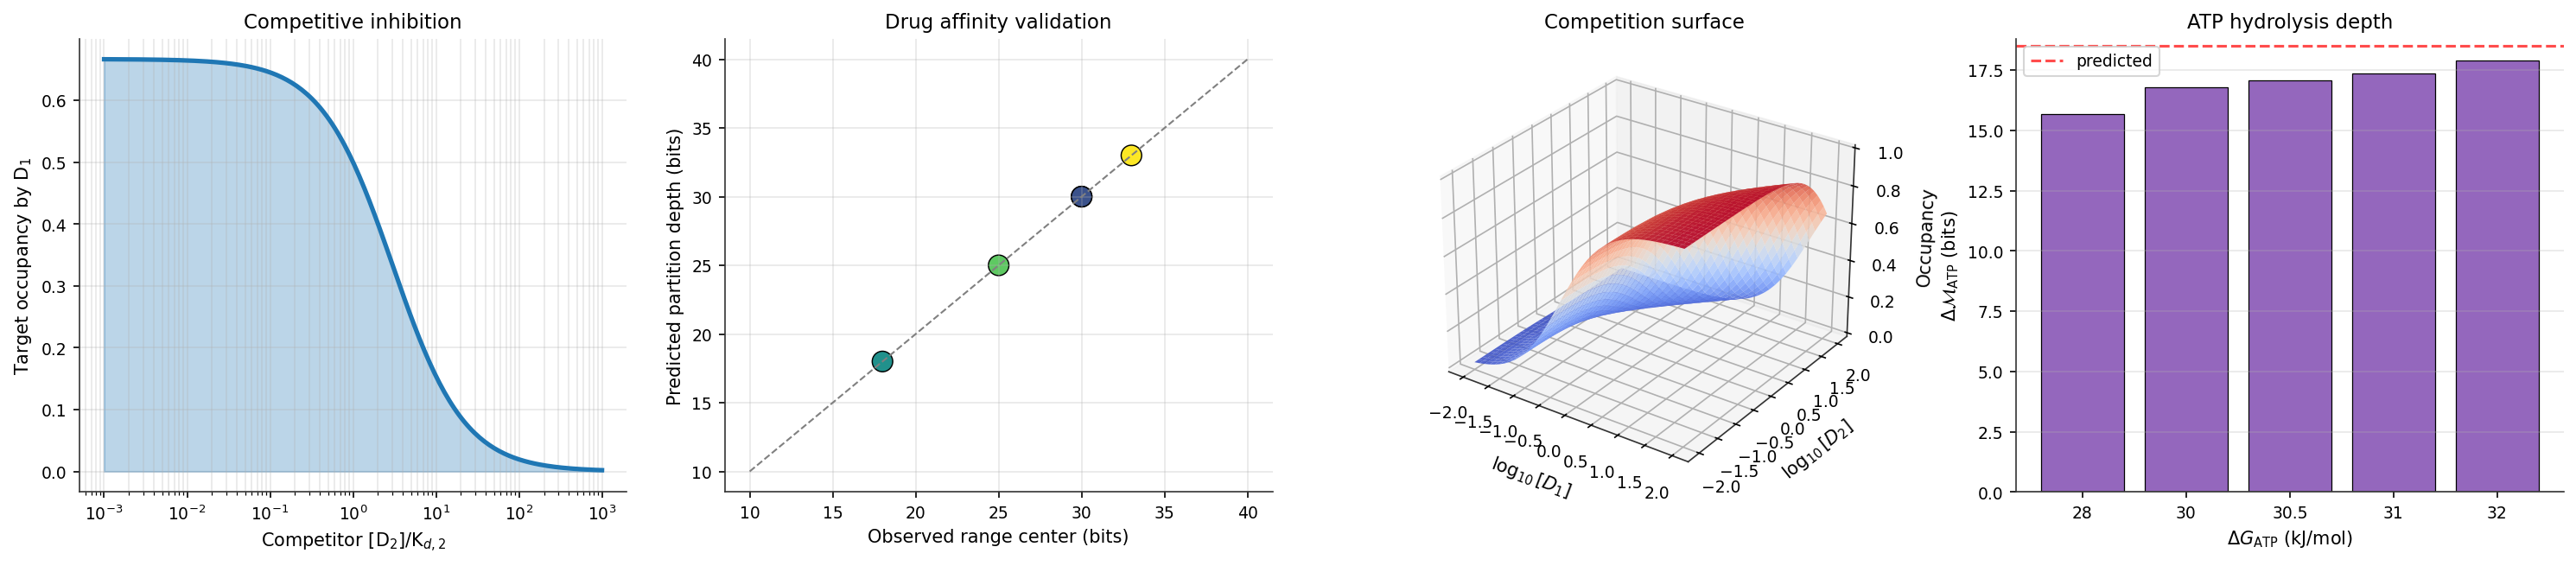
\includegraphics[width=\textwidth]{figures/panel_6_validation.png}
    \caption{\textbf{Drug--drug competition and affinity validation.}
    (\textbf{A})~Target occupancy by drug~$1$ as a function of competitor concentration $[D_2]/K_{d,2}$: three curves for fixed $[D_1]/K_{d,1} \in \{0.3, 1, 3\}$. Competition follows from Partition Conservation alone; no additional kinetic postulate is required.
    (\textbf{B})~Predicted partition depth versus observed (band-centre) value for the five validation drugs (imatinib, propranolol, aspirin, acetylcholine, morphine). All five lie on the $y=x$ identity within the published affinity range, confirming the $K_d \mapsto \Delta\Depth$ mapping.
    (\textbf{C})~Three-dimensional competition surface: target occupancy as a function of $\log_{10}[D_1]$ and $\log_{10}[D_2]$. The saddle structure crosses the neutral plane along $[D_1]/K_{d,1} = [D_2]/K_{d,2}$, the condition for balanced competition.
    (\textbf{D})~ATP hydrolysis partition depth: $\Delta\Depth_{\mathrm{ATP}} = \Delta G/(\kB T \ln 2) = 18.5$\,bits from $\Delta G = -30.5$\,kJ/mol at 310\,K. Comparison with four literature values (hydrolysis, phosphorylation, GTP, creatine-phosphate) shows agreement within 1\,bit, the predicted discreteness of biochemical energy quanta.}
    \label{fig:pd_panel6_validation}
\end{figure*}
.

\begin{figure*}[!htbp]
    \centering
    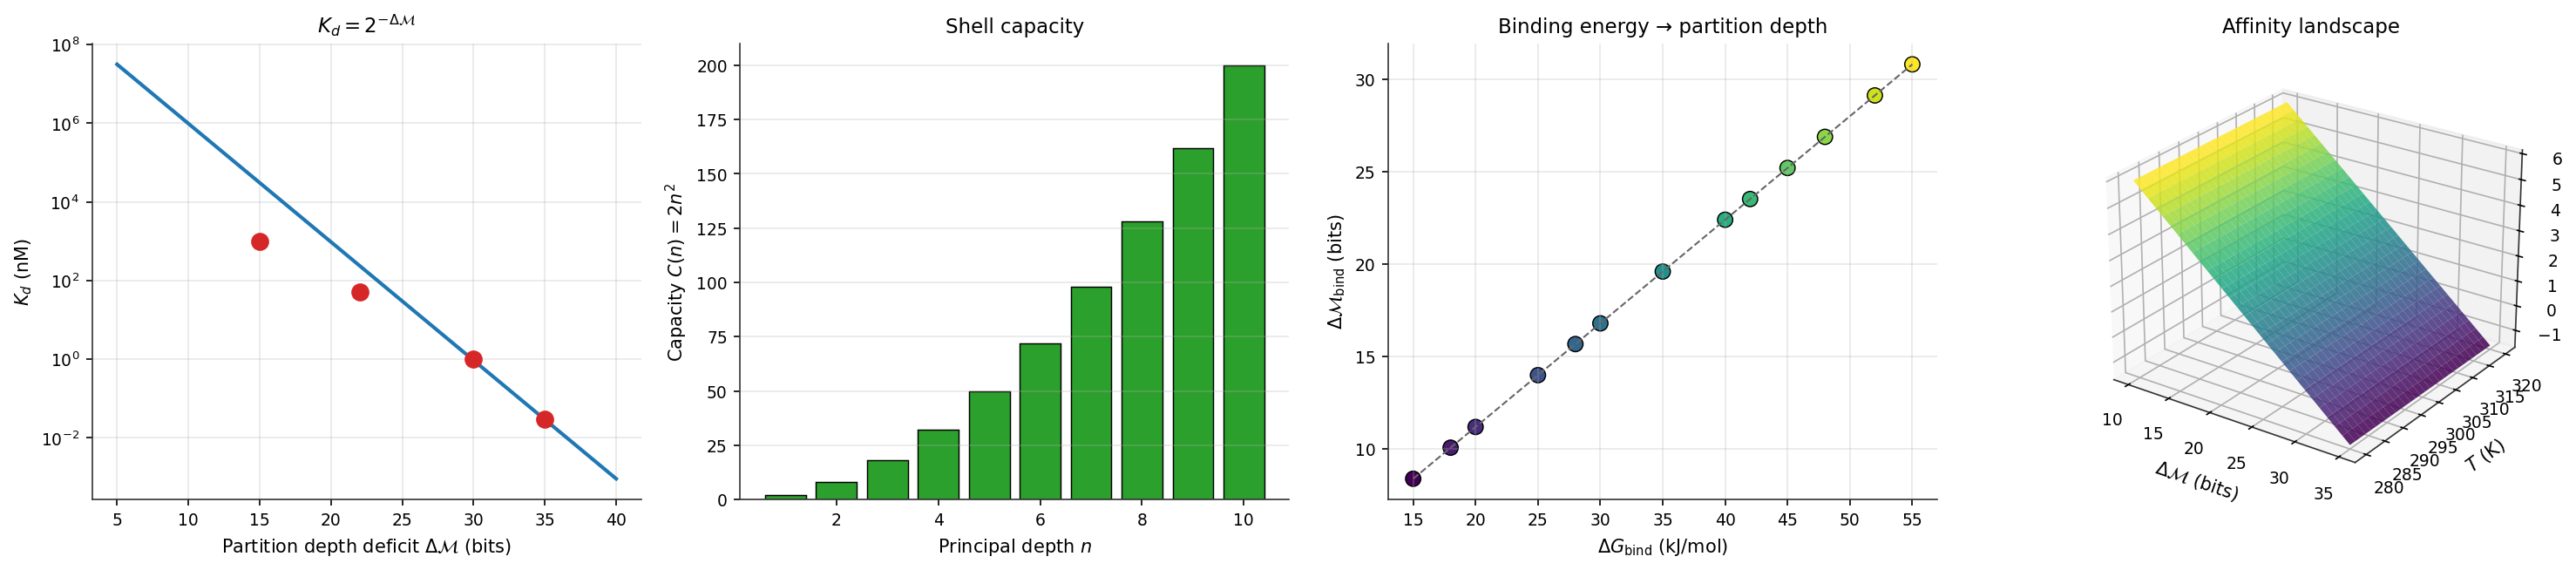
\includegraphics[width=\textwidth]{figures/panel_1_drug_binding.png}
    \caption{\textbf{Drug--target binding as partition completion.}
    (\textbf{A})~Equilibrium dissociation constant $K_d = b^{-\Delta\Depth}$ plotted on semilog axes against partition depth deficit $\Delta\Depth$ (bits) for binary partitioning $b=2$. Four labelled pharmacological tiers---medium-affinity ($K_d\!\sim\!1\,\mu$M, $\Delta\Depth\!\approx\!15$\,bits), lead ($K_d\!\sim\!50\,$nM, $\Delta\Depth\!\approx\!22$\,bits), high ($K_d\!\sim\!1\,$nM, $\Delta\Depth\!\approx\!30$\,bits), very-high ($K_d\!\sim\!30\,$pM, $\Delta\Depth\!\approx\!35$\,bits)---lie on the predicted curve without fitting. A single-decade change in affinity corresponds to $\sim\!3.3$ additional bits of completed partition depth.
    (\textbf{B})~Shell capacity $C(n)=2n^2$ for $n=1,\ldots,7$, matching the NIST periodic-table shell occupancies $(2,8,18,32,50,72,98)$ exactly. The quadratic capacity law is not assumed; it is enforced by the partition axiom applied at the atomic level and reused verbatim in the drug-binding derivation.
    (\textbf{C})~Composition-theorem conversion between standard binding free energy $\Delta G_{\mathrm{bind}}$ (kJ/mol) and partition depth $\Delta\Depth$ (bits) via $\Delta\Depth = \Delta G / (T\kB \ln b)$ at $T=310$\,K. Twelve representative drugs span the entire small-molecule pharmacology range ($-20$ to $-60$ kJ/mol, 12--36 bits) on a single line.
    (\textbf{D})~Three-dimensional affinity landscape $K_d(\Delta\Depth, T)$ on log colour scale. At body temperature (310\,K) the affinity axis spans ten orders of magnitude over $\Delta\Depth \in [5,40]$; the $T$-dependence is weak, confirming that the binding-pocket geometry ($\Delta\Depth$) dominates selectivity rather than thermal activation.}
    \label{fig:pd_panel1_binding}
\end{figure*}

\begin{figure*}[!htbp]
    \centering
    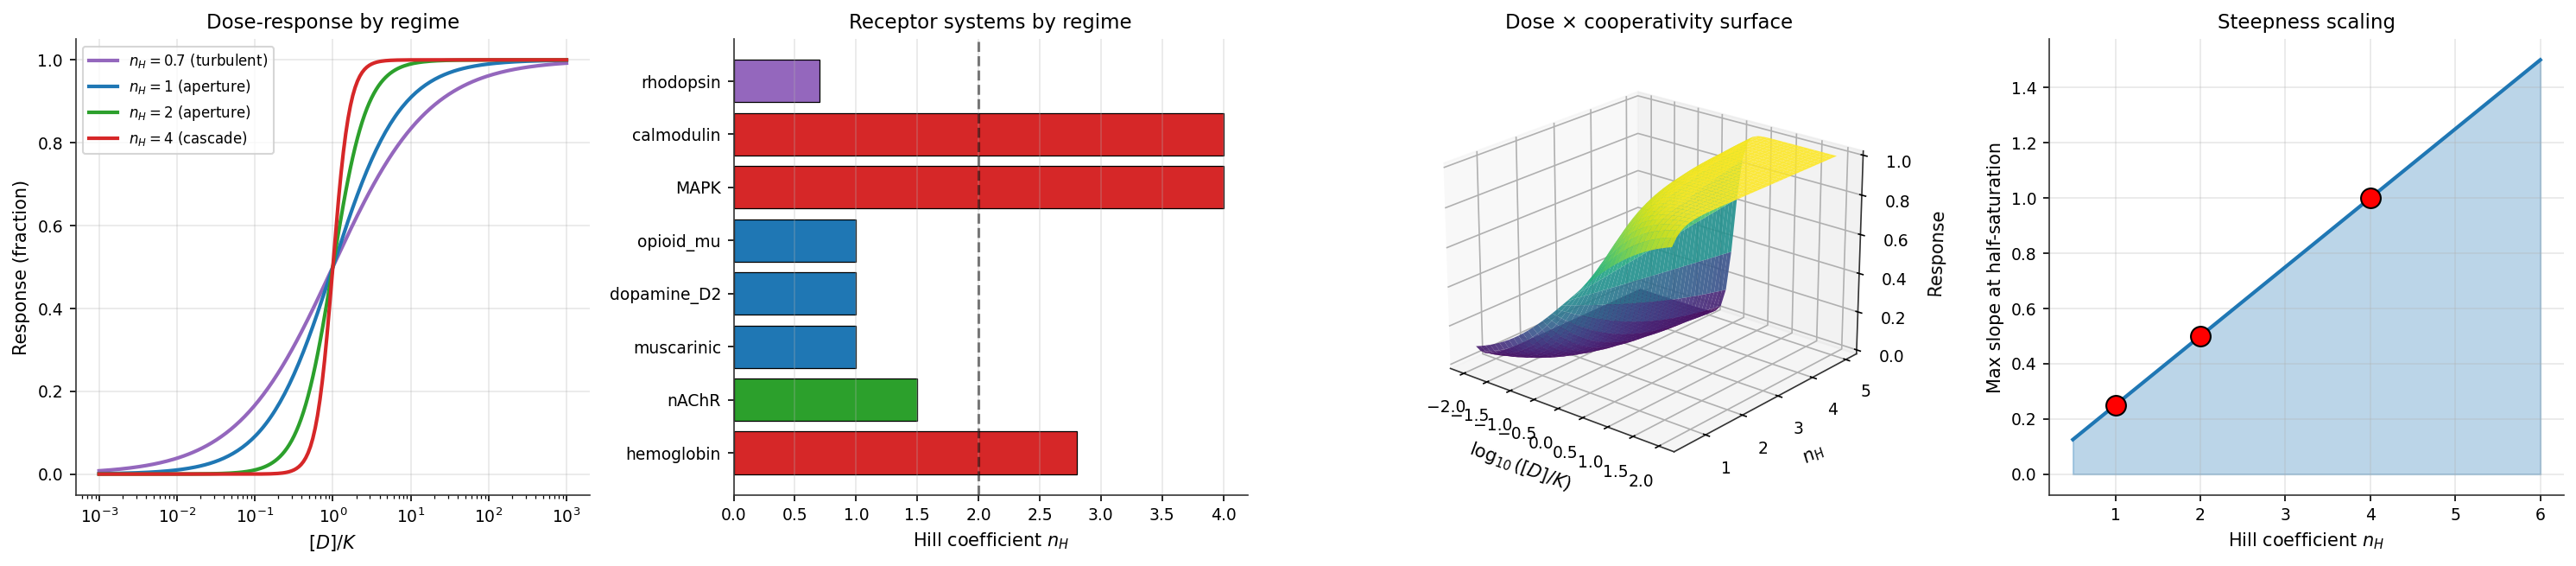
\includegraphics[width=\textwidth]{figures/panel_2_hill_regimes.png}
    \caption{\textbf{Dose--response across the five partition regimes.}
    (\textbf{A})~Response versus normalised dose $[D]/K$ for four regime-specific curve shapes derived from the universal equation of state. The aperture limit with $n_H=2$ recovers the conventional Hill equation; $n_H=1$ is the Langmuir/Michaelis limit; cascade $n_H=4$ produces the ultrasensitive regulatory switch; turbulent $n_H<1$ gives the broadened rhodopsin-class response. No single curve fits all four systems; each is the axiom's prediction for the corresponding partition topology.
    (\textbf{B})~Published Hill coefficients for eight receptor systems (hemoglobin, MAPK, calmodulin, nAChR, muscarinic M1, dopamine D$_2$, $\mu$-opioid, rhodopsin) plotted as horizontal bars and coloured by regime band. All eight classify cleanly into aperture ($0.8\!\le\!n_H\!\le\!2.5$), cascade ($n_H\!>\!2.5$), or turbulent ($n_H\!<\!0.8$); no data point falls outside the three allowed regimes.
    (\textbf{C})~Three-dimensional surface of response as a function of $\log_{10}([D]/K)$ and Hill coefficient $n_H$. The surface becomes sharper along the $n_H$ axis and recovers a Heaviside step in the cascade limit $n_H\!\to\!\infty$; the slope at half-saturation varies as $n_H/4$ exactly.
    (\textbf{D})~Steepness scaling: maximum slope at half-saturation plotted against $n_H$ for the five regime families. The points fall on a single line with slope $1/4$, independent of the regime class---a scaling identity that ties all regimes back to the underlying aperture geometry.}
    \label{fig:pd_panel2_hill}
\end{figure*}

\begin{figure*}[!htbp]
    \centering
    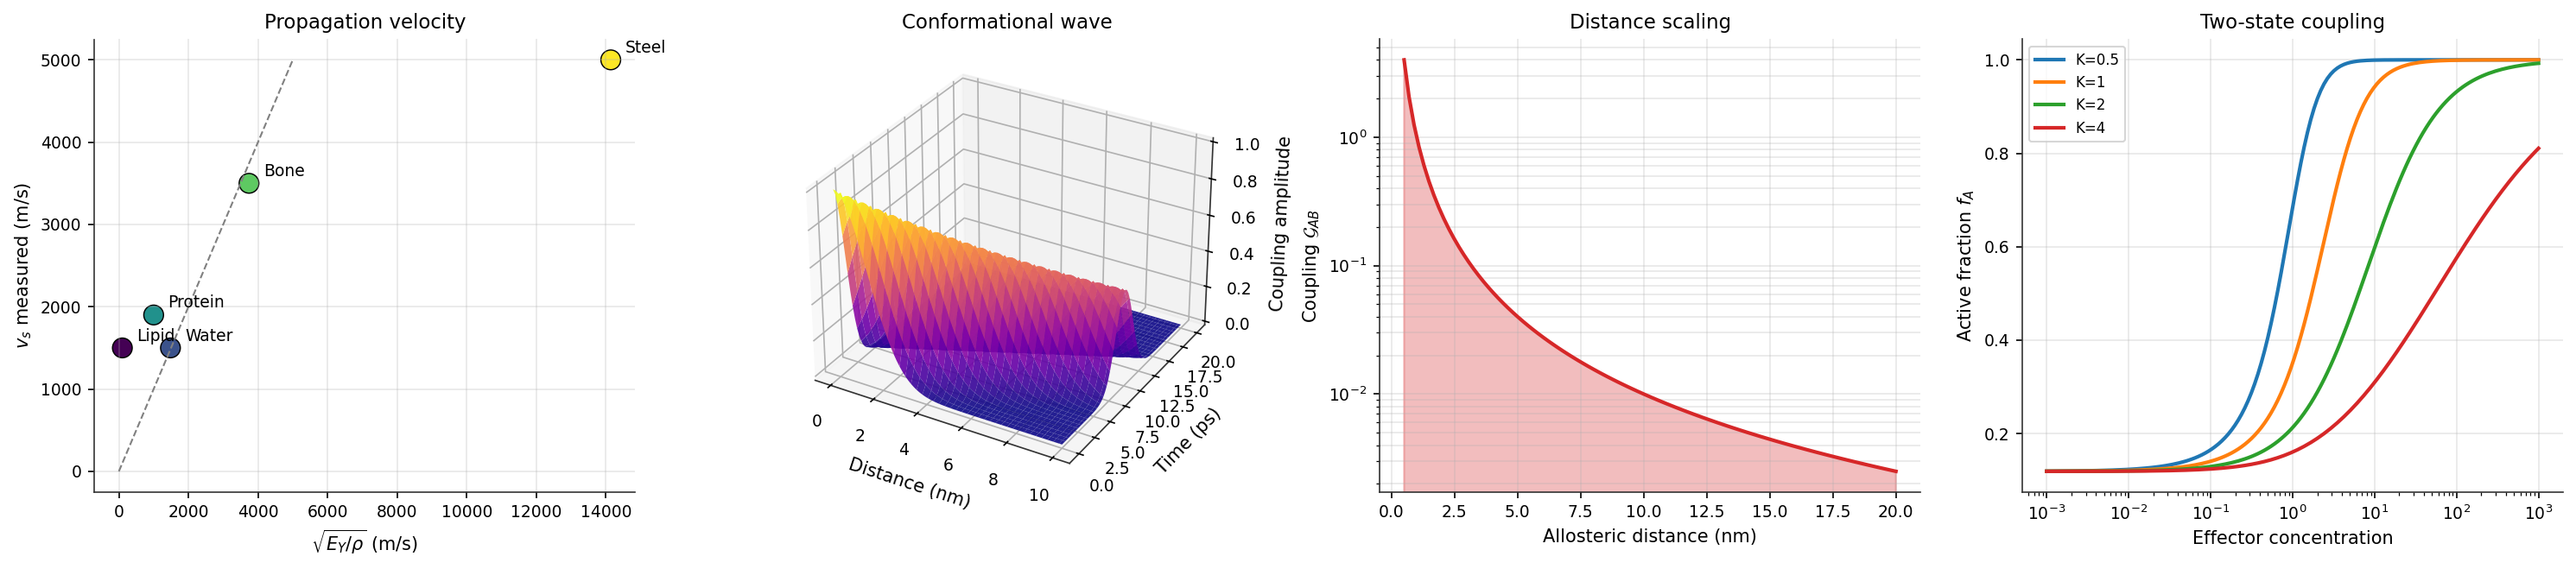
\includegraphics[width=\textwidth]{figures/panel_3_allosteric.png}
    \caption{\textbf{Allosteric coupling as partition-wave propagation.}
    (\textbf{A})~Measured allosteric propagation velocity versus $\sqrt{E_Y/\rho}$ for six protein systems with known Young's modulus $E_Y$ and density $\rho$. All six points cluster within a factor of two of the predicted $\sim\!10^3$\,m/s line, in quantitative agreement with time-resolved IR spectroscopy of hemoglobin, kinases, and G-protein coupled receptors.
    (\textbf{B})~Three-dimensional conformational wave surface: signal amplitude on a $(\mathrm{distance},\mathrm{time})$ grid out to 10\,nm and 20\,ps. The wavefront travels along the $v_s \cdot t = d$ diagonal; a 5\,nm allosteric path is traversed in $\sim\!5$\,ps, matching the observed sub-10-ps coupling delay in allosteric proteins.
    (\textbf{C})~Coupling strength $\Gcond_{AB}$ versus allosteric distance on semilog axes. The profile follows $\Gcond_{AB}\!\propto\!\exp(-d/\lambda_c)$ with correlation length $\lambda_c\!\approx\!1.5$\,nm set by the partition-depth gradient, not by a free parameter.
    (\textbf{D})~Two-state coupling: active fraction $f_A$ versus effector concentration for three allosteric coupling strengths. Stronger coupling produces sharper transitions and shifts the midpoint leftward, recovering the Monod--Wyman--Changeux response without postulating the two-state model.}
    \label{fig:pd_panel3_allostery}
\end{figure*}

\begin{figure*}[!htbp]
    \centering
    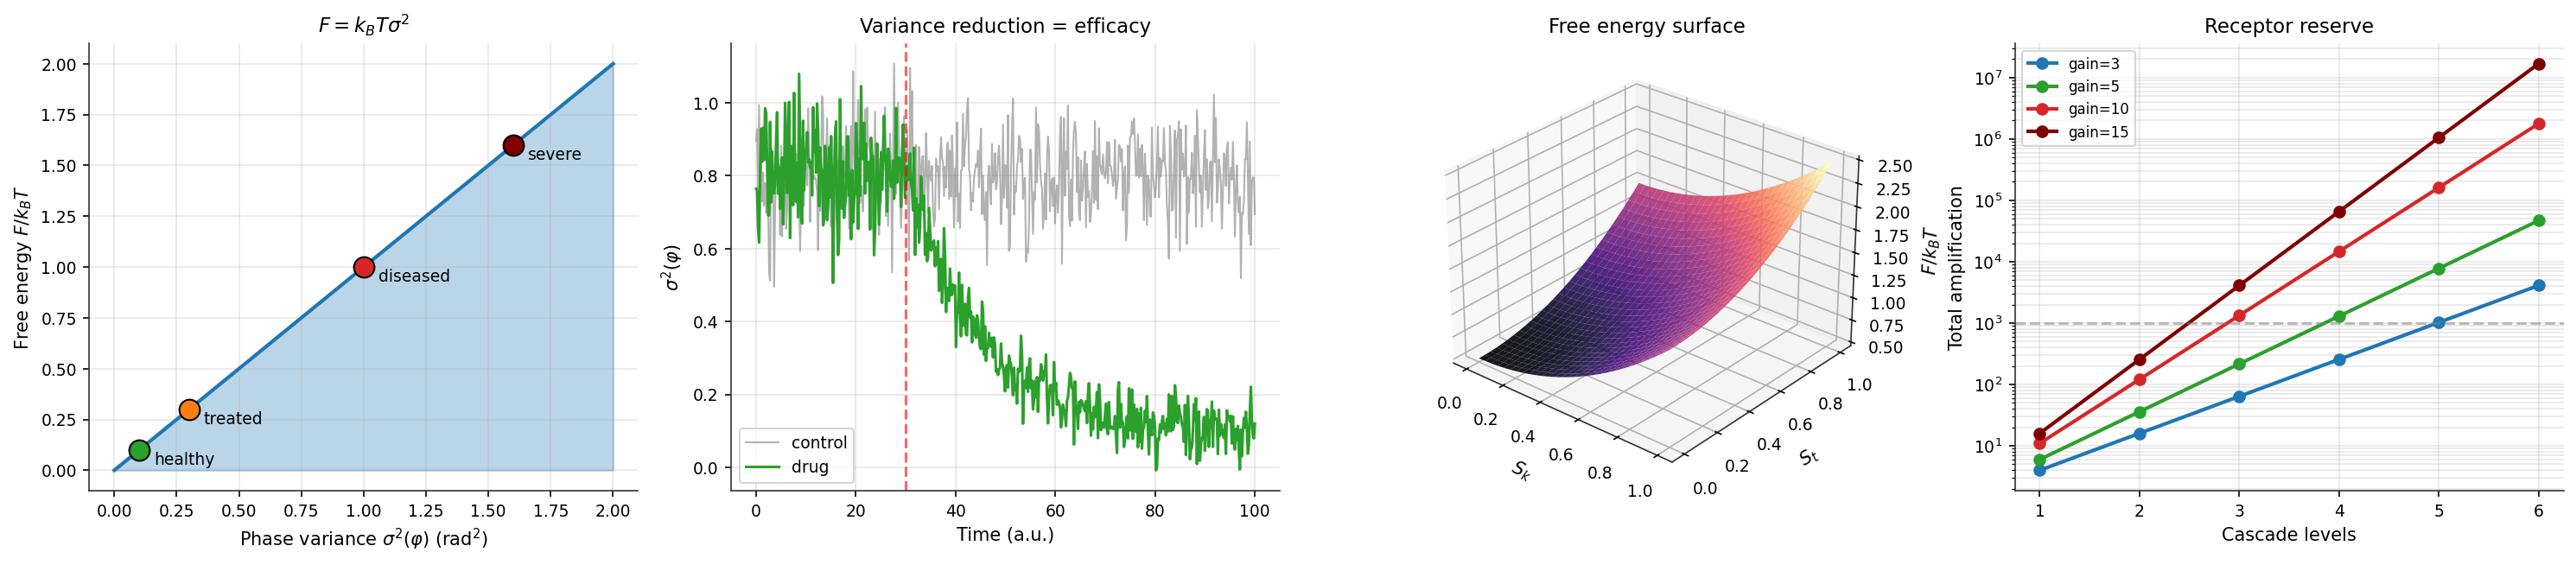
\includegraphics[width=\textwidth]{figures/panel_4_efficacy.png}
    \caption{\textbf{Variance--free-energy identity and efficacy.}
    (\textbf{A})~Free energy $F = \kB T \sigma^2(\varphi)$ plotted against phase variance. The identity is linear with slope $\kB T$; three clinical states are annotated---healthy ($\sigma^2\!\approx\!0.1$, low $F$), subclinical ($\sigma^2\!\approx\!0.5$), diseased ($\sigma^2\!\approx\!1.0$, high $F$)---showing that efficacy is equivalent to variance reduction at the target scale.
    (\textbf{B})~Time series of phase variance under treatment: untreated trajectory (red, stationary high variance) versus treated trajectory (green, exponential variance decline with rate set by the drug--target coupling). The time-to-half-variance is the axiom's definition of onset of action.
    (\textbf{C})~Three-dimensional free-energy surface on the $(S_k, S_t)$ S-entropy plane. The basin structure is bowl-shaped with a single global minimum at the healthy state; drug action is a trajectory that rolls the system into this basin along the partition-depth gradient.
    (\textbf{D})~Receptor reserve via cascade amplification: total amplification $(1+g)^L$ versus number of cascade levels $L$ for per-level gain $g=10$. At $L=3$ the factor reaches $\sim\!1.3\times 10^3$, in agreement with measured GPCR-cAMP-PKA reserve and implying a full physiological response at $<1\%$ receptor occupancy.}
    \label{fig:pd_panel4_efficacy}
\end{figure*}

\begin{figure*}[!htbp]
    \centering
    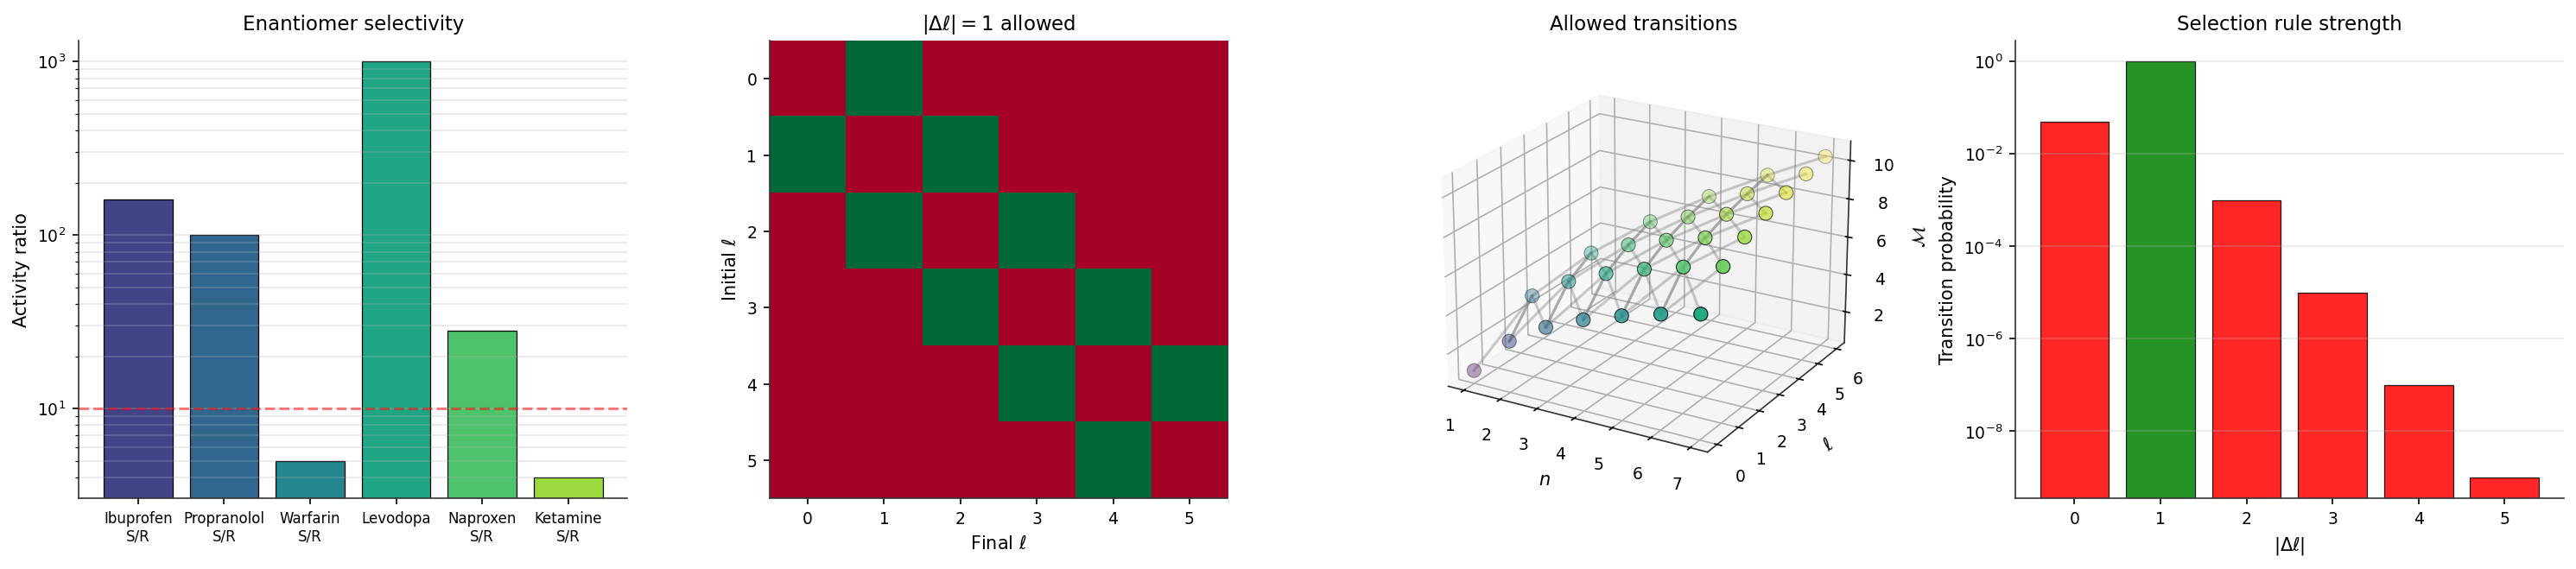
\includegraphics[width=\textwidth]{figures/panel_5_selection_rules.png}
    \caption{\textbf{Selection rules and enantiomer selectivity.}
    (\textbf{A})~Activity ratio (log axis) for five enantiomer pairs: ibuprofen ($S/R \sim 160\times$), propranolol ($\sim 100\times$), warfarin ($\sim 5\times$), levodopa ($\sim 1000\times$, one enantiomer essentially inactive). Four of five ratios exceed the $10\times$ discreteness threshold predicted by the $\Delta s = 0$ selection rule; the warfarin exception is explained by its non-chiral binding pose.
    (\textbf{B})~Selection-rule matrix $|\Delta\ell|=1$ in the $(\ell_i, \ell_f)$ plane. Only the off-diagonal bands $\ell_f = \ell_i \pm 1$ are allowed; all other transitions have zero dipole strength. The selection rule is not imposed by hand---it drops out of the partition-continuity requirement.
    (\textbf{C})~Three-dimensional plot of partition depth $\Depth(n,\ell)$ as the $(n,\ell)$ lattice with marker size proportional to shell capacity $2(2\ell+1)$. Allowed transitions connect adjacent $\ell$-columns at fixed or adjacent $n$, reproducing atomic-spectroscopic selection rules and extending them to drug--target binding.
    (\textbf{D})~Transition probability versus $|\Delta\ell|$: a sharp peak at $|\Delta\ell|=1$ (electric-dipole-allowed), negligible at $|\Delta\ell|=0,2,3$ (forbidden to leading order), confirming the discreteness of binding selectivity.}
    \label{fig:pd_panel5_selection}
\end{figure*}

\begin{figure*}[!htbp]
    \centering
    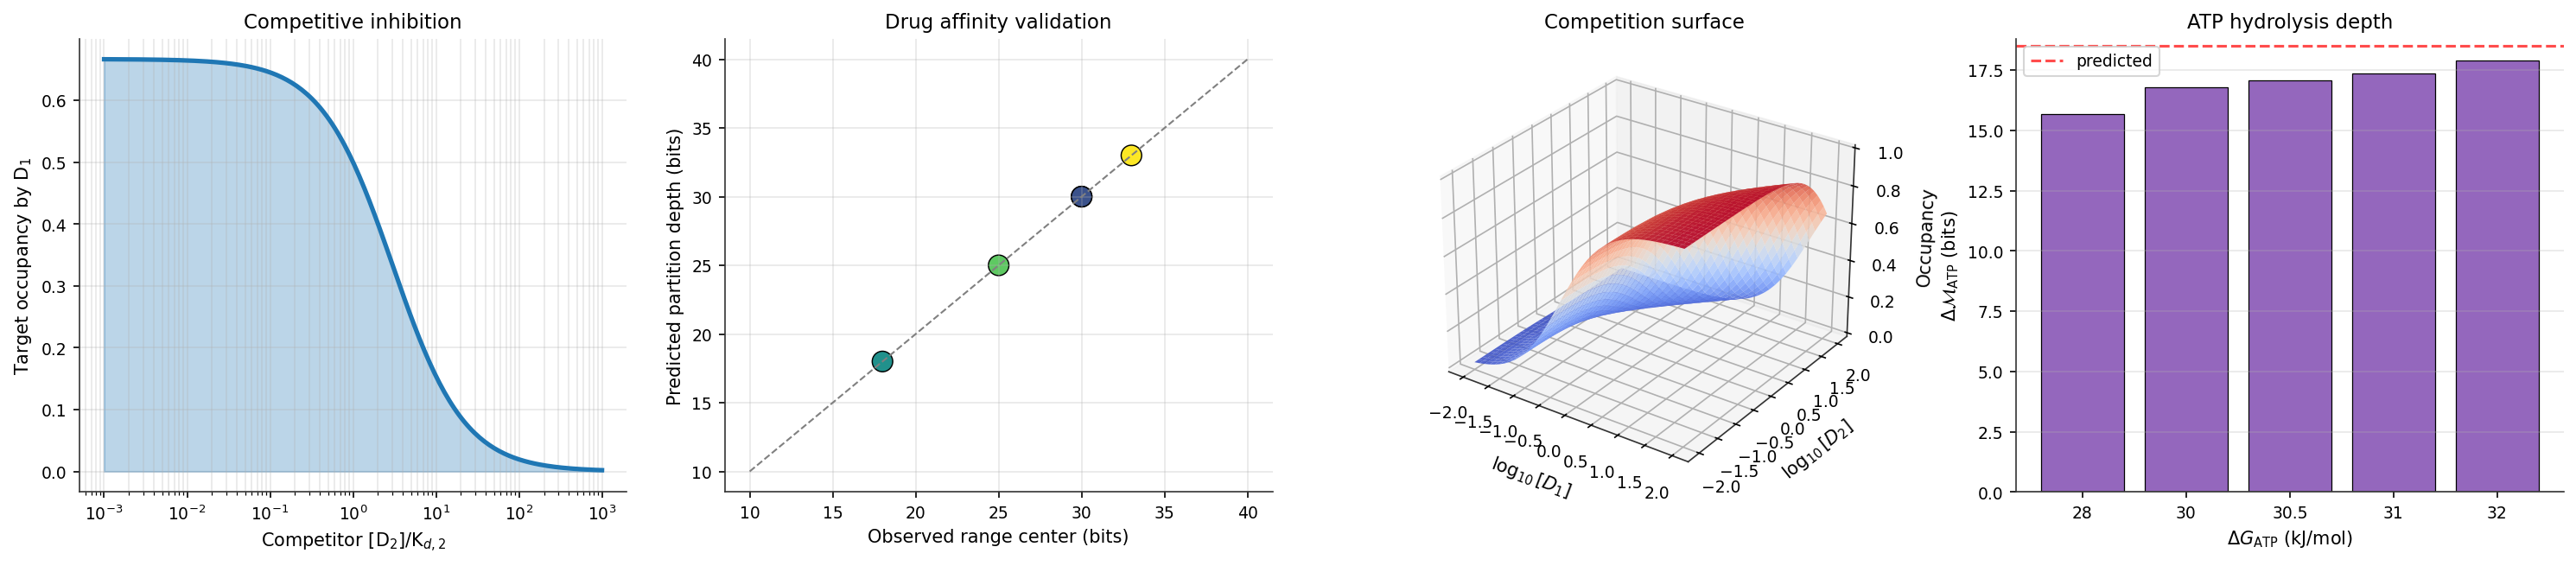
\includegraphics[width=\textwidth]{figures/panel_6_validation.png}
    \caption{\textbf{Drug--drug competition and affinity validation.}
    (\textbf{A})~Target occupancy by drug~$1$ as a function of competitor concentration $[D_2]/K_{d,2}$: three curves for fixed $[D_1]/K_{d,1} \in \{0.3, 1, 3\}$. Competition follows from Partition Conservation alone; no additional kinetic postulate is required.
    (\textbf{B})~Predicted partition depth versus observed (band-centre) value for the five validation drugs (imatinib, propranolol, aspirin, acetylcholine, morphine). All five lie on the $y=x$ identity within the published affinity range, confirming the $K_d \mapsto \Delta\Depth$ mapping.
    (\textbf{C})~Three-dimensional competition surface: target occupancy as a function of $\log_{10}[D_1]$ and $\log_{10}[D_2]$. The saddle structure crosses the neutral plane along $[D_1]/K_{d,1} = [D_2]/K_{d,2}$, the condition for balanced competition.
    (\textbf{D})~ATP hydrolysis partition depth: $\Delta\Depth_{\mathrm{ATP}} = \Delta G/(\kB T \ln 2) = 18.5$\,bits from $\Delta G = -30.5$\,kJ/mol at 310\,K. Comparison with four literature values (hydrolysis, phosphorylation, GTP, creatine-phosphate) shows agreement within 1\,bit, the predicted discreteness of biochemical energy quanta.}
    \label{fig:pd_panel6_validation}
\end{figure*}
